% !TEX root = defense_index.tex

\begin{displayquote}
\begin{centering}
\begin{singlespace}
\textbf{Scarecrow}:
\par
The sum of the square roots of any two sides of an isosceles triangle is equal to the square root of the remaining side. Oh joy! Rapture! I got a brain! How can I ever thank you enough?
\par
\textbf{The Wizard of Oz}:
\par
You can't.
\par
\end{singlespace}
\end{centering}
\end{displayquote}

%%%%%%%%%%%%%%%

This chapter introduces the nature and use of \acp{EEG} in clinical and research settings. Clinical \acp{EEG} are used by clinicians to make diagnostic decisions in accordance with their education and training. In research settings algorithms strive to replicate the performance of clinicians through statistical modeling guided by clinician annotated data. Together these two groups are increasing our ability to discern the meaning of \ac{EEG} signals.

This dissertation will examine the suitability of \acp{IV} as a mathematical tool for allowing researchers to replicate clinician performance on \acp{EEG}. \acp{IV} have shown promise with respect to classification and clustering of speech signals in terms of accent, age, context, gender, and language via its feature transformation process. This type of discrimination would be beneficial to understanding the phenomena that produce \ac{EEG} waveforms. The \ac{IV} technique is introduced in depth along with the necessary criteria to evaluate it against other algorithm based discrimination techniques.

%%%%%%%%%%%%%%%%%%%%%%%%%%%%%
%%%%%%%%%%%%%%%%%%%%%%%%%%%%%
% SECTION -  Electroencephalograms
%%%%%%%%%%%%%%%%%%%%%%%%%%%%%
%%%%%%%%%%%%%%%%%%%%%%%%%%%%%
\section{Electroencephalograms}
\label{sec:eeg}

An \ac{EEG} records the electrical activity of the brain. The captured voltage signals represent the firing of neurons involved with all aspects of a brain's functionality. Through the use of \acp{EEG} we can see how the brain functions on an operational level \cite{Coan2004}, interprets stimuli \cite{Doppelmayr1998a}, and changes due to diseases and disorders \cite{Porjesz2005}. The applications of \acp{EEG} are primarily limited by the ability to link recorded activity to the underlying physiological condition.

A clinician's ability to annotate \ac{EEG} recordings utilizes their knowledge of the relationship between waveforms and physiological conditions. An accurate diagnosis cannot be made from waveforms only as the clinician must consider the subject's history and the recording conditions of the \ac{EEG}. In many cases spatial and temporal properties must be considered when assess for specific conditions related to different regions of the brain and similarities between waveforms.

Depending on application, \ac{EEG} signals require radically different signal processing techniques for separating or decoding them. For example, whereas seizure and sleep waveforms are distinct and easily separable \cite{Markand2003}, EEG signals in BCI applications are typically subtle and require custom spatial and/or temporal filters \cite{Makeig2012}. This changes the discrimination techniques when dealing with \ac{BCI} to spatial and temporal features \cite{Blankertz2007a,Kasabov2015}. Auditory and visual stimulus response \cite{Picton1992} have distinct spatial patterns as well adding to the diversity of \ac{BCI} waveform morphology \cite{Kindermans2014}.

To distinguish spatial and temporal features, \acp{EEG} are partitioned via channels and epochs. As discussed previously, the channels are a representation of the electrodes, shaped by filtering and montages. Epochs segment the data as a function of time, typically on the order of seconds. Clinician and algorithm based approaches both rely on these techniques, but in different ways. Clinicians will review \acp{EEG} using epochs on the order of tens of seconds \cite{Warby2014, Silber2007}, while algorithms operate on epochs of seconds \cite{Wulsin2011,Kindermans2014}.

One of the main diagnostic applications of \acp{EEG} is the classification of seizures \cite{Wulsin2011}. Seizures represent excessive electrical activity within a region of the brain which manifest as high energy waveforms. The study of sleep is also an active research area given the occurrence of seizures during sleep and sleep's impact on brain health \cite{Radha2014}. When recording for seizure and sleep activity a substantial amount of background activity is also captured. This enables enables an analysis of overall brain function, like the presence of \ac{ADHD} in children\cite{Loo2008a}. Adult \acp{EEG} also provide insight into numerous conditions such as alcoholism \cite{Porjesz2005}, Alzheimer's Disease \cite{Jeong2004}, brain development \cite{Segalowitz2010}, emotion \cite{Coan2004}, and stress \cite{Lupien2007}.

In a research setting, \acp{BCI} promote a deeper understanding of brain functionality by allowing those with disabilities to communicate \cite{Picton1992} and regain functionality \cite{Ajiboye2017}. \acp{BCI} highlight the ability of algorithms to classify waveforms beyond the capabilities of clinicians. These computer-driven methods enabled the development of novel applications in clinical monitoring, video games \cite{Lance2012}, and bio-metrics \cite{Fazli2011a}. All of these use real-time classification which is not in the purview of clinicians. Specifically, bio-metrics provide the ability to dissect the facets of \ac{EEG} that differentiate one person from another. This is a level of discrimination that clinicians cannot attain and serves needs far beyond clinical settings in hospitals.

Moving \acp{EEG} outside of hospitals has expanded the potential applications of \acp{EEG}\cite{Liao2012}. It is easier to produce \ac{EEG} datasets for experiments, but even with these advances there are few publicly available datasets. Those datasets available having varying levels of documentation and labeling related to conditions, subjects, and tasks. In addition, the sampling rates and number of channels have no definitive standards which furthers the disparate nature of the recordings. Recording in non-clincial environments often increases the likeliehood of artifacts, but even under ideal clinical conditions artifacts are still present requiring pre-processing\cite{Mahajan2015,Nolan2010}.

The following sections focus on the process and techniques of collecting \ac{EEG} signals from a brain. Electrode configuration and montages are two important tools clinicians use when making a diagnosis from a recording. They provide flexibility to the clinician, but hamper the ability of algorithms to validate themselves on similar data. The experimental datasets are also introduced to highlight the difficulties of working with publicly available data.

%%%%%%%%%%%%%%%%%%%%%%%%%%%%%%%%%%%%%%%%%%%%%%%%
\subsection{Properties of Electroencephalograms}

An \ac{EEG} is comprised of multiple surface/scalp electrode channels capturing the continuous signals generated by the brain. These signals represent the aggregated neuronal activity of the cortical neurons in immediate proximity to each electrode. Each channel maps to a specific electrode that is placed on the scalp, extracranially, or in the case of \acp{IEEG} directly on the brain's surface. Electrode placement for extra-cranial recordings follows a standardized layout, \cref{fig:eeg_1020layout}, based upon relative distances \cite{Jurcak2007}. Intra-cranial electrodes are high density electrode grids that are placed directly on the brain region of interest. This increases the complexity of the electrode and the data collected which excludes them from this work, but there is no theoretical reason \acp{IV} could not operate on such signals.

%%%%%%%%%%%%%%%%%%%
\begin{figure}[ht]
\centering
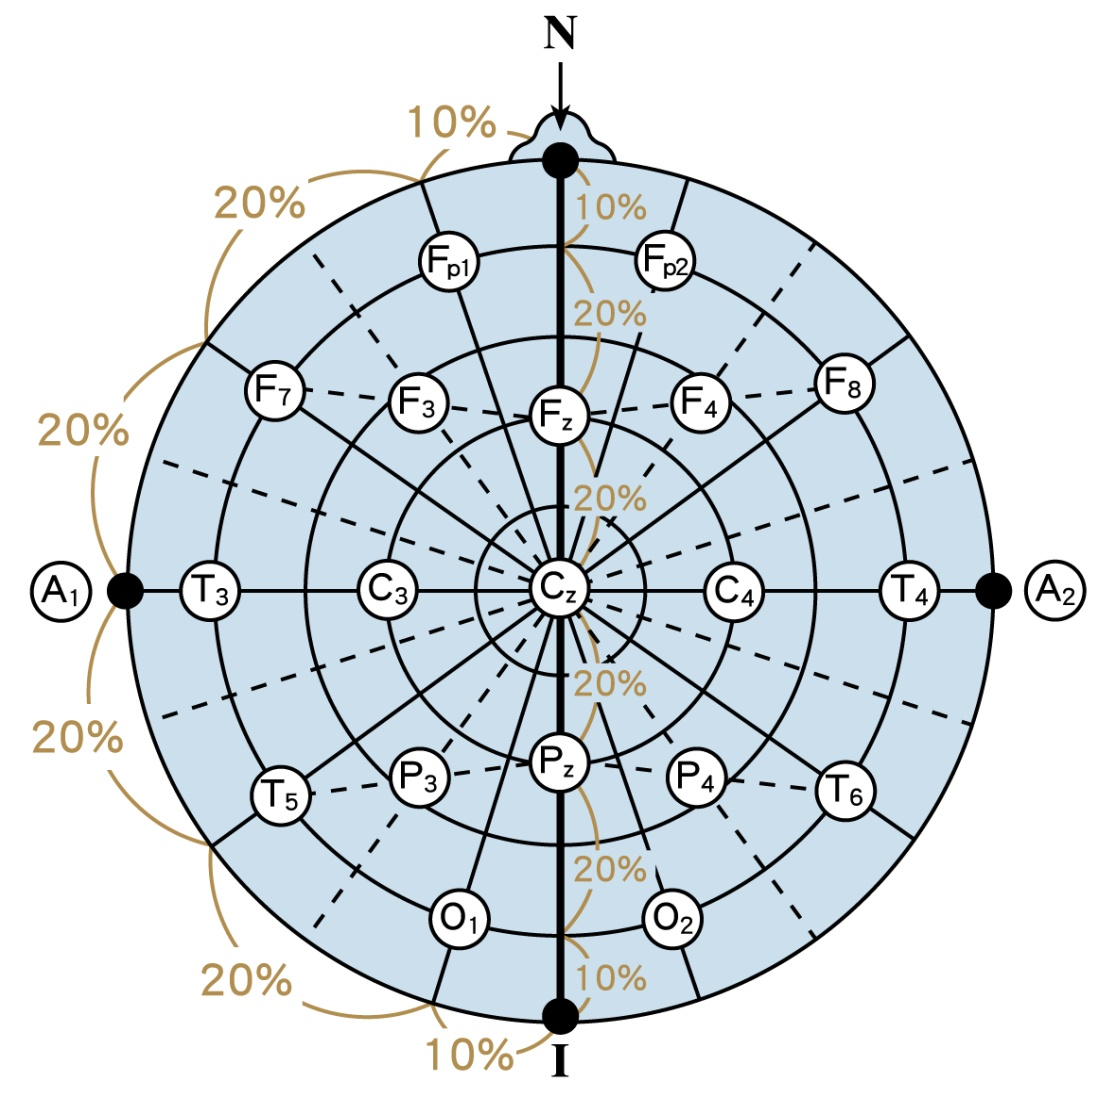
\includegraphics[width=0.75\linewidth,keepaspectratio]{1020_layout}
\caption[10-20 EEG Configuration]{The 10-20, 10-10, and 10-5 layouts for \ac{EEG} electrodes utilize a proportional unit of measure for the distribution of electrodes. The first number represents the distance of the electrodes from the nasion and inion and the second represents the space between subsequent electrodes. With this approach adding electrodes does not change the location of the previous electrodes. Image sourced from \cite{Cheng2011}.}
\label{fig:eeg_1020layout}
\end{figure}
%%%%%%%%%%%%%%%%%%%

The electrode configuration dictates the number of channels in the recording. To visual these signals clinicians view them indirectly as \textit{montages}, a differential electrode configuration. Montages, \cref{tab:eeg_montage}, can be configured to be referential to a common ground electrode, neighboring electrode, or a contralateral electrode. These configurations aid in the diagnostic process by calling attention to patterns of behavior in the recording. Below are three sets of montages for a system with eighteen channels\footnote{Taken from: \url{https://www.acns.org/UserFiles/file/EEGGuideline3Montage.pdf} }.

%%%%%%%%%%%%%%%%%%%
\begin{table}[ht]
\caption{Table of EEG Montages}
\centering
\begin{tabular}{ c c c c c }
\toprule
Channel & \makecell{Longitudinal\\Bipolar} & \makecell{Transverse\\Bipolar} &
\makecell{Referential to\\Ground(Ear)} \\
\midrule
1 & Fp1-F7	& F7-Fp1		& F7-A1		\\
2 & F7-T3		& Fp1-Fp2		& T3-A1		\\
3 & T3-T5		& Fp2-F8		& T5-A1		\\
4 & T5-O1		& F7-F3		& Fp1-A1		\\
5 & Fp1-F3	& F3-Fz		& F3-A1		\\
6 & F3-C3		& Fz-F4		& C3-A1		\\
7 & C3-P3		& F4-F8		& P3-A1		\\
8 & P3-O1		& T3-C3		& O1-A1		\\
9 & Fz-Cz		& C3-Cz		& Fz-A1		\\
10 & Cz-Pz	& Cz-C4		& Pz-A2		\\
11 & Fp2-F4	& C4-T4		& Fp2-A2		\\
12 & F4-C4	& T5-P3		& F4-A2		\\
13 & C4-P4	& P3-Pz		& C4-A2		\\
14 & P4-O2	& Pz-P4		& P4-A2		\\
15 & Fp2-F8	& P4-T6		& O2-A2		\\
16 & F8-T4	& T5-O1		& F8-A2		\\
17 & T4-T6	& O1-O2		& T4-A2		\\
18 & T6-O2	& O2-T6		& T6-A2		\\
\bottomrule
\end{tabular}
\label{tab:eeg_montage}
\end{table}
%%%%%%%%%%%%%%%%%%%

Montages serve to improve the clarity of each channel. Theoretically they do not impact the content of the channels, but evaluating such a claim is beyond the immediate focus of this work. Filtering of the channel data, before or after inclusion in a montage, is necessary to separate signals into the five standard \ac{EEG} frequency bands, \cref{tab:eeg_band}. Signals between 2Hz to 80Hz represent the spectrum commonly viewed by clinicians\footnote{While this is the dominant spectrum of interest, research using \acp{IEEG} indicates activity at higher frequencies ($>$500Hz) may contain relevant discriminatory data related to seizures \cite{Blanco2010}.}. For many conditions  the frequency range of activity is critical in signal classification. Motor activity signals dominate the alpha band \cite{Dahne2014}, while the stages of sleep affect all but the gamma band \cite{Schluter2012}. 

%%%%%%%%%%%%%%%%%%%
\begin{table}[ht]
\caption[EEG Frequency Bands]{Table of EEG Frequency Bands. *When dealing with motor cortex signals it is common to encounter the Mu band (9-11Hz) which resides within the Alpha band.}
\centering
\begin{tabular}{ c c c }
\toprule
Band Name & Frequency Range (Hz) & Attributes \\
\midrule
Delta & 1-3 & \makecell{Brain health,\\deep sleep} \\
Theta & 4-7 & \makecell{ADHD rhythms,\\relaxation} \\
Alpha* & 8-12 & \makecell{motor activity,\\alertness} \\
Beta & 13-30 & \makecell{anxiety,\\focus} \\
Gamma & 31-80 & \makecell{REM sleep,\\stress} \\
\bottomrule
\end{tabular}
\label{tab:eeg_band}
\end{table}
%%%%%%%%%%%%%%%%%%%

%%%%%%%%%%%%%%%%%%%%%%%%%%%%%%%
\subsection{Available Datasets}

There are a number of publicly available \ac{EEG} datasets \footnote{The University of California San Diego maintains a website, \url{https://sccn.ucsd.edu/~arno/fam2data/publicly_available_EEG_data.html}, indexing many of the publicly available datasets.}. These datasets are developed for specific studies independently of each other resulting in a wide variation of data content and format. Their data formats range across \ac{EDF}, Matlab formatted files, and raw text files. The data content differs in terms of electrodes, sampling rates, and the studied phenomena.

This work applies to the \ac{PNET} dataset and the \ac{TUHEEG} dataset. These datasets have been standardized to utilize the same 20 channel \ac{TCP} montage. In addition the \ac{TUHEEG} dataset contains annotations from multiple sources providing robust labeling of events. This helps control for variation between the \ac{BCI} focused \ac{PNET} dataset and predominantly seizure focused \ac{TUHEEG} dataset.

%%%%%%%%%%%%%%%%%%%%%%%%%%%%%%%%%%%%%%%%%%%%%%%%%%%%%
\subsubsection{Temple University Hospital EEG Corpus}

The \ac{TUHEEG} dataset contains over 25,000 \ac{EEG} studies and their associated neurological evaluations taken from \ac{TUH} in Philadelphia, Pennsylvania \cite{Obeid2016a}. Each patient's records present with different electrode configurations and sampling rates. The curated corpus uses a common 22 channel montage, \ac{TCP} shown in \cref{fig:eeg1020}, for all subjects with a static sample rate of 250Hz.

%%%%%%%%%%%%%%%%%%%
\begin{figure}[ht]
\centering
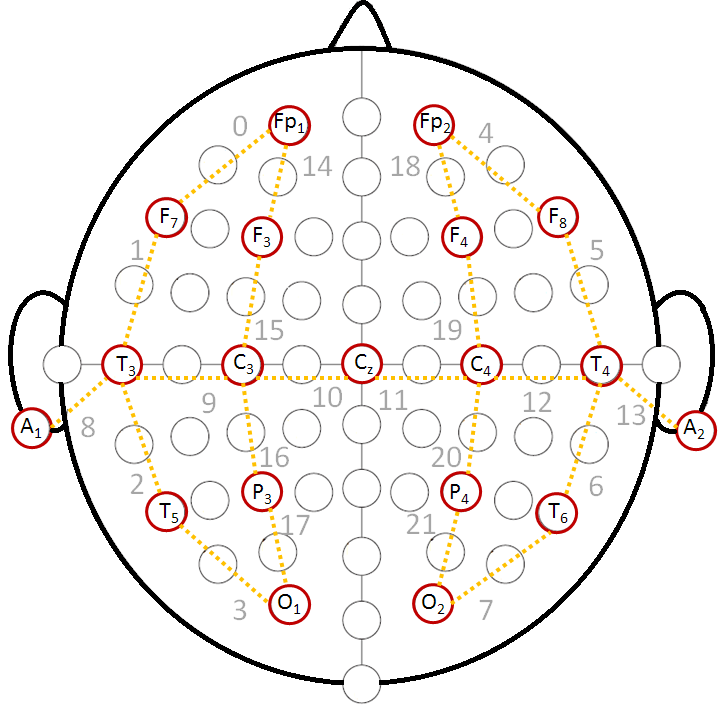
\includegraphics[width=0.75\linewidth,keepaspectratio]{figure3}
\caption[The \acs{TCP} Montage Layout]{The \ac{TCP} Montage channels (red) used by the TUH EEG corpus is overlaid on the \ac{PNET} channel layout. Each montage link (orange) is assigned an index for storing the montage channel (gray) data in the corpus. The proper 10-20 channel names (black) are provided for the montage channels.}
\label{fig:eeg1020}
\end{figure}
%%%%%%%%%%%%%%%%%%%

The dataset contains longitudinal results of patients receiving continuing care at the hospital. These include multiple same patient sessions in a given day or sessions spaced out over a number of years. \ac{TUH} treats patients of varying backgrounds (age, gender, diagnosis) providing breadth to the data. Recording profiles at \ac{TUH} range from 23 to 32 electrodes with sampling rates of 250Hz, 256Hz, 400Hz, or 512Hz \cite{Obeid2016a}. Computerized \ac{EEG} analysis is complicated by the fact that even small variations in electrode placement can hamper generalizations between subjects. This problem is exacerbated when datasets from disparate sources are combined.

%%%%%%%%%%%%%%%%%%%%%%%%%%%%%%%%%%%%%%%%%%%%%%%%%%%%%%%%%%%%%
\subsubsection{PhysioNet EEG Motor Movement/Imagery Database}

The \ac{PNET} data contains 109 subjects following computer prompted motion/motion imagery trials at the New York State Department of Health's Wadsworth Center \cite{Schalk2004}. The recordings present 64 electrodes following a 10-20 layout sampled at 160Hz. From this base layout, the data is converted to the same 22 channel \ac{TCP} montage used by the \ac{TUHEEG}.

Each subject performs two calibration trials (resting eyes open and resting eyes closed) and twelve task driven trials. The four tasks consist of opening/clenching the (1) left or (2) right first and opening/clenching both (3) fists or (4) feet as a physical and imaginary movement. A trial consists of 30 tasks that alternates between rest and motor tasks. The calibration trials last for one minute and the motor trials last for two minutes, providing 26 total minutes of subject data. The data is publicly available through the \ac{PNET} website \cite{Goldberger2000}.

There are 12 total motion tasks representing three groups. These groups consist of 4 repeated trials creating natural cohorts of grouped trials: \{3, 7, 11; 4, 8, 12; 5, 9, 13; 6, 10, 14\}. \cref{fig:pNetEx} shows the layout of tasks within each trial and their associated grouping. The major experiments utilize these trial level cohorts and the unique 109 subjects to develop I-Vectors for discrimination on the trial and subject level.

%%%%%%%%%%%%%%%%%%%
\begin{figure}[ht]
\centering
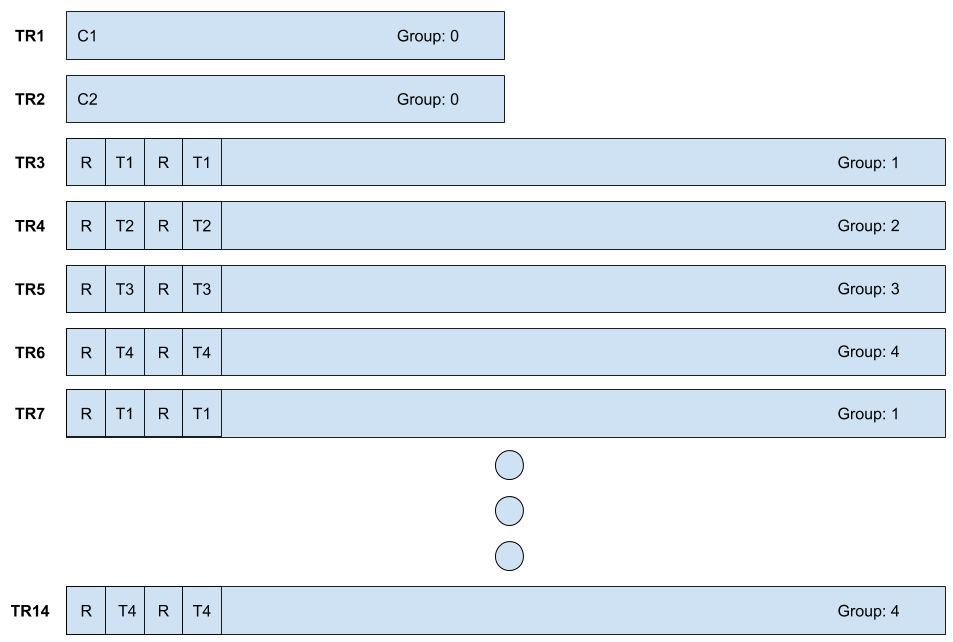
\includegraphics[width=0.75\linewidth,keepaspectratio]{figure4}
\caption[PhysioNet Trial Composition]{Each subject from the PhysioNet data set completed 14 trials. Two of these trials (TR1 and TR2) are one minute calibrations trials of resting eyes open and resting eyes closed. The remaining 12 trials are two minute recordings of a predefined sequence consisting of a task state and resting state. With four tasks states, each task is repeated three times producing four groups of task related trials. These trial groups provide the basis for cohort retrieval on the trial level.}
\label{fig:pNetEx}
\end{figure}
%%%%%%%%%%%%%%%%%%%

%%%%%%%%%%%%%%%%%%%%%%%%%%%%%
%%%%%%%%%%%%%%%%%%%%%%%%%%%%%
% SECTION -  Applications and Classifications
%%%%%%%%%%%%%%%%%%%%%%%%%%%%%
%%%%%%%%%%%%%%%%%%%%%%%%%%%%%
\section{Applications and Classification of Electroencephalograms}

The techniques used by algorithms and clinicians to classify and cluster \ac{EEG} data are unique. An algorithm's foundation is informed by the knowledge of clinicians via their annotated data. A clinician's knowledge comes from their experience treating patients and their formal education. The algorithms are dependent on the clinicians' annotations to build their knowledge base, making them susceptible to clinician bias. Clinicians are skeptical of algorithm performance because it does not match clinical performance. As algorithms attempt to improve their classification they are competing against experts in a field that is still being understood. Progress is slow because it is difficult for algorithms and clinicians to be confidant in the reasoning of their classifications. This makes it difficult to produce accurate testing datasets given the competing views on what are accurate annotations.

Clinicians annotate \acp{EEG} recordings to diagnose their patient. Typical clinical recordings are 20 minutes or more depending on the nature of the assessment. Each recording is accompanied by a detailed \ac{EEG} report \cite{Epstein2006}. These reports must document the subject, the testing carried out, and address the \textit{clinical questions}\footnote{Clinical questions are posed prior to testing by the clinician. They serve to inform the clinician about the patient, their condition, and what outcomes are possible. As an example, if a patient has seizures while sleeping it would be necessary to determine the location of these seizures, their severity, and how such seizures compare to other patient populations. These would all be questions answered through \ac{EEG} recordings.}. The interpretation of an \ac{EEG} recording is the main criteria when affirming a diagnosis, but must be supported by evidence indicating the recording is normal or abnormal\cite{Kaplan2013}.

This annotation and reporting process relies on the clinician's ability to review segments of the full recording for waveforms relevant to the clinical questions. A clinically relevant interpretation of the patient's condition may not be forthcoming without reviewing the reports of other tests and/or subjects \cite{Epstein2006}. This meta-analysis across subjects is a clustering process informed by medical records and annotations. However, the \ac{EEG} reports focus on determining if the results inform the clinical questions or not \cite{Kaplan2013}. This does not require all relevant phenomena to be annotated, as only enough data must be collected to affirm a position. As such a clinician's ability to cluster could be hampered by their ability to annotate, which is suggested by tracking a clinician's ability to reproduce classifications \cite{Halford2017}.

In contrast, an algorithm's approach to annotation is much more broad. Depending on the desired outcome, algorithms can perform a normal/abnormal classification \cite{Lopez2015}, annotate specific epochs \cite{Wulsin2011} or combine these approaches to classify \ac{EEG} recordings \cite{Schluter2012}. Each of these classification techniques is a subset of the classification approach used by clinicians. Performance of these algorithms is measured against gold standards generated from training data annotated by clinicians \cite{Wulsin2011,Warby2014}. The goal is develop algorithms capable of mirroring clinical performance which limits the strength of the algorithms to the strength of the clinicians.

Depending on the output of these algorithms, they are capable of clustering \ac{EEG} recordings in a way clinicians cannot replicate. The ability to infer similarity of waveforms, epochs, and entire recordings across subjects is important in the development of robust \ac{BCI} \cite{Lotte2010a} and bio-metric applications\cite{Campisi2014}. In this area algorithms exceed the ability of clinicians by shifting how \ac{EEG} recordings are evaluated through novel channel and feature selection \cite{Rocca2013,Brigham2010,Fraschini2015}.

Specifically, bio-metric algorithms can determine the similarity of one subject to another \cite{Campisi2014,VanBeijsterveldt2002}. This makes bio-metric subject verification the closest analog to \acp{IV}, but they are not limited to subject comparisons. Instead they offer the ability to discriminate on multiple facets of the data without needing the same extent of bio-metric pre-processing \cite{Dehak2011a}. This makes their application to \ac{EEG} recordings interesting as \acp{IV} may be capable of bridging classification between algorithms and clinicians.

%%%%%%%%%%%%%%%%%%%%%%%%%%%%%%%%%%%%%
\subsection{Clinician Classification}

For clinically annotated \ac{EEG} recordings it is important that common terminology was used when describing the waveforms. Without a shared vocabulary \ac{EEG} reports would be ineffectual for diagnostics and documentation\cite{Epstein2006}. Gaspard et al.\cite{Gaspard2014} tested 49 clinicians' agreement on terminology by asking them 409 questions about 37 pre-selected \ac{EEG} waveforms. Their protocol removed the need of the clinician to find the epochs, enabling them to focus on each clinician's ability to describe the contents of each pre-selected epoch.

Each clinician's background varied in terms of experience (2-15+ years) and training (adult or pediatric neurology). While the epochs were sourced from only critical care patients exhibiting \acp{PLED}, \acp{GPED}, seizures, and other rhythmic activity. The epochs were presented using a modified biploar montage with a bandpass filter spanning 1Hz-70Hz. From these epochs, clinicians made \emph{categorical assessments} based upon the presence of a seizure and dominant morphologies and \emph{ordinal assessments} based upon the physical properties on the signals (sharpness, amplitude, frequency, etc). The overall and inter-rater agreement of the clinicians is presented in \cref{tab:gaspard}.

%%%%%%%%%%%%%%%%%%%
\begin{table}[ht]
\caption[EEG Terminology Agreement]{Each terminology item, aside from Seizure, could be classified with multiple responses. Fast Activity could be yes, no, or no applicable while Phases were 1, 2, 3, $>$3, not applicable forcing the clinicians to articulate their classifications. Agreement specifies the percentage of waveforms classified correctly. The $\kappa$ score indicates the amount of inter-rater agreement, see \ref{append-cohen}.}
\centering
\begin{tabular}{l c r}
\toprule
Terminology Item & Agreement (\%) & \makecell{$\kappa$ statistic\\(95\% CI)} \\
\midrule
Categorical					&	&	\\
Seizure 						& 93.3 & 91.1 (90.6-91.6) \\
Main Term 1 					& 91.3 & 89.3 (89.1-89.6) \\
Main Term 2 					& 85.2 & 80.3 (79.4-81.2) \\
Triphasic Morphology 			& 72.9 & 58.2 (56.1-60.2) \\
Plus + Modifier 				& 49.6 & 33.7 (32.4-35.1) \\
Any +	 					& 59.3 & 19.2 (17.5-20.9) \\
+ Fast Activity 				& 71.9 & 65.5 (64.4-66.7) \\
+ Rhythmic Activity 			& 76.5 & 67.4 (66.5-68.3) \\
+ Spike or Sharply Contoured & 83.9 & 81.8 (81.2-82.5) \\
\midrule
Ordinal						&	&	\\
Sharpness 					& 91.5 & 84.8 (84.3-85.2) \\
Absolute Amplitude 			& 96.5 & 94.0 (93.8-94.2) \\
Relative Amplitude 			& 71.8 & 66.4 (65.3-67.4) \\
Frequency 					& 97.8 & 95.1 (94.9-95.2) \\
Phases 						& 89.9 & 83.0 (82.6-83.4) \\
Evolution 					& 65.6 & 21.0 (19.7-22.2) \\
\bottomrule
\end{tabular}
\label{tab:gaspard}
\end{table}
%%%%%%%%%%%%%%%%%%%

In 12 of the 15 categories, the clinicians' exceeded an agreement of 70\% and 7 of the 15 showed near- perfect (0.81-1.00) $\kappa$ statistics. The categories with the lowest agreement and weakest $\kappa$ statistics were categorical classifications. With only 3 morphologies reporting $\kappa$ below substantial (0.61-0.80), the results suggest the clinicians perform well as a group. Yet, those three categories indicated a universal blind spot that would be passed on to an algorithm built from this annotated data. Since the contents of epochs were known, this showed how difficult it was for clinicians to agree on labeling of wavefroms.

These biases likely existed because clinicians were evaluated on their annotations indirectly. Their diagnoses were not solely based on a single event in the \ac{EEG}, but rather the sum of the recordings in conjunction with the patient's medical history. In Halford et al. \cite{Halford2017} the importance of detecting \acp{ET} was found to be critical for diagnosing epilepsy. Failing to annotate some of the \acp{ET} does not change the diagnosis because the clinicians were primed to make a decision about epilepsy. Individually the 18 tested clinicians were unable to produce a Gwet agreement coefficient\footnote{The Gwet's AC2 is an alternative to $\kappa$ statistics for quantifying inter-rater similarity, but is bounded over the same range \cite{Gwet2012}.} over 0.50 with the rest of the group. This indicated a weak agreement among the clinicians. Despite varying levels of certification and years of practice, there were no distinct indicators of what characteristics represented a better annotator.

The difficulty in producing accurate annotations with respect to others existed at the intersection of finding the waveforms and then correctly labeling them. These problems were documented to various degrees when clinicians' annotation skills were tested on critically ill patients \cite{Gerber2008}, patients exhibiting seizures \cite{Grant2014, Halford2015}, comatose cardiac patients \cite{Westhall2015}, and sleeping subjects \cite{Silber2007}. The results of such studies highlighted problems with clinician inter-rater and intra-rater agreement as a function of the type of \ac{EEG} data.

%%%%%%%%%%%%%%%%%%%%%%%%%%%%%%%%%%%%%%%%%%%%%%%
\subsubsection{Clinician Inter-rater Agreement}

The previous section discussed this broadly and with the benefit of the waveforms being pre-selected. However, when clinicians were asked to annotate longer epochs the discrepancies shift from clinical knowledge to issues of annotation style. Their inter-rater agreement was the ability of one clinician's classification to agree with one or more other clinicians.

A pedantic instance of this was seen in \cref{fig:halford_match} where two clinicians labeled seizure events \cite{Halford2015}. In the highlighted section, Rater B identified two discrete events while Rater A labels them as one event. Each of them notices at least 4 other seizure events, but their agreement was weakened because of their three misidentified events. Behavior such as this further complicated how to quantify agreement and disagree based upon duration of said annotations.

%%%%%%%%%%%%%%%%%%%
\begin{figure}[ht]
\centering
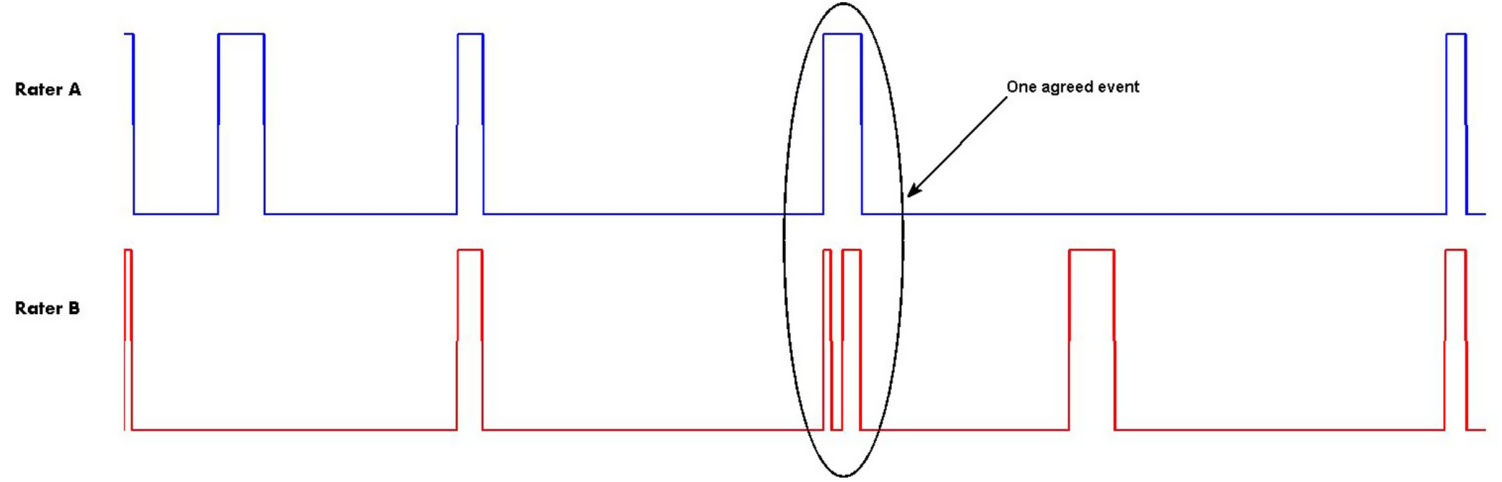
\includegraphics[width=0.9\linewidth,keepaspectratio]{halford_match}
\caption[Inter-rater annotation matching]{An example of how open ended annotation styles lead to inconsistencies in evaluating the accuracy of inter-rater agreements.}
\label{fig:halford_match}
\end{figure}
%%%%%%%%%%%%%%%%%%%

This example came from Halford et al.\cite{Halford2015} where the agreement of 8 clinicians was test on 30 one hour \ac{ICU} \ac{EEG} recordings from 20 seizure patients. Each clinician was asked to label \acp{PD} events, a strong indicator of a seizure, and true seizure events. The resultant $\kappa$ statistics for the group were 0.58, moderate, for seizures and 0.38, fair, for \ac{PD}. These results highlighted the difficulty in finding consensus by suggesting it surpassed their background and experience. There was a clear issue in how clinicians selected waveforms in the recordings, which resulted in less data being included in any gold standard.

Gerber et al.\cite{Gerber2008} conducted a study with a more expansive classification list than Halford et al.'s by expanding the available labels and varying the amount of available data. Two data sets, split into epochs of 10 seconds and epochs $>$20 minutes, were built from 11 subjects with convulsive seizures, status epilepticus\footnote{Status epilepticus is the categorization of a person's state when seizures occur close together or occur for a prolonged duration($>$5 minutes).}. The results, \cref{tab:gerber_inter}, showed the clinicians' consensus was stronger on the shorter epochs (0.04-0.68) than the longer epochs (0.07-0.44).

%%%%%%%%%%%%%%%%%%%
\begin{table}[ht]
\caption[Gerber's Long Versus Short Segment Classification]{Results of classification using segments of 10 seconds and $>20$ minutes in length. Five clinicians annotated the shorter epochs and all seven clinicians annotated the longer epochs. The $\kappa$ statistics for both datasets are reported along with the raw agreement percent for the 20min epoch dataset.}
\centering
\begin{tabular}{l c c c}
\toprule
Term & \makecell{10s Epoch \\ Kappa} & \makecell{20min Epoch \\ Kappa} & \makecell{20min Epoch\\ Agreement ($\%$)}\\
\midrule
Rhythmic/periodic vs. excluded			& 0.68 & 0.44 & 82\\
Localization							& 0.49 & 0.42 & 66\\
Morphology							& 0.39 & 0.37 & 69\\
Frequency								& 0.34 & 0.27 & 78\\
``Quasi'' vs. Not						& 0.04 & 0.07 & 57\\
``Frontally Predominant'' vs. Not		& 0.40 & 0.08 & 68\\
+ vs. Not								& 0.12 & 0.08 & 62\\
\bottomrule
\end{tabular}
\label{tab:gerber_inter}
\end{table}
%%%%%%%%%%%%%%%%%%%

The most critical labels (rhythmic/periodic vs. excluded, localization, and morphology) exceed 65\% agreement, but only rhythmic/periodic exceeds 80\%. This meant that on average each clinician failed to recognize 20\% to 35\% of what the other clinicians annotated. Without definitively labeled data it was impossible to determine if the 35\% gap is due to false positives or false negatives. Such knowledge could be used to determine if they were over-jealous or overly-shrewd in their annotations. However, it was possible their performance was impeded by alignment issues similar to those seen in Halford et al.'s work. The results otherwise suggested that the clinicians agree at a moderate to fair level which was enough to make accurate medical decisions, but not sufficient from which to train algorithms.

Gerber et al.'s best reported inter-rater agreement was inline with Halford et al.'s. This trend persisted in the work of Grant et al.'s work \cite{Grant2014}. Their study evaluated the agreement of 6 clinicians (adult and pediatric neurologists) classifying 7 categories (status epilepticus, seizure, epileptiform discharges w/ and w/o slowing, slowing, normal, uninterpretable) of waveforms in 150 30 minute \ac{EEG} epochs. Each clinician reviewed a unique set of 150 epochs from the full dataset's 300 30-minute epochs. Over the 15 inter-rater pairs, their inter-rater $\kappa$ scores ranged from 0.29 to 0.62 suggesting fair to substantial agreement among the pairs.

%%%%%%%%%%%%%%%%%%%
\begin{table}[ht]
\centering
\caption[Inter-rater agreement of clinicians]{Inter-rater agreement for the 15 clinician pairs observed by Grant. The pair averaged $\kappa$ score is 0.44 giving the overall agreement as moderate.}
\begin{tabular}{l c}
\toprule
Reader Pair & $\kappa$ score \\
\midrule
AB	&	0.43\\
AC	&	0.52\\
AD	&	0.37\\
AE	&	0.37\\
AF	&	0.50\\
BC	&	0.48\\
BD	&	0.41\\
BE	&	0.37\\
BF	&	0.29\\
CD	&	0.49\\
CE	&	0.56\\
CF	&	0.62\\
DE	&	0.48\\
DF	&	0.35\\
EF	&	0.42\\
\bottomrule
\end{tabular}
\label{tab:grant_inter}
\end{table}
%%%%%%%%%%%%%%%%%%%

Westhall et al. \cite{Westhall2015} had a smaller subject pool, 4 clinicians, but asked them to evaluate \ac{EEG} recordings for specific to \emph{Prespecified \ac{EEG} patterns}, \emph{Background \ac{EEG}}, or \emph{Periodic or rhythmic patterns}. Each $>20$ minute recording was drawn from a pool of 103 comatose cardiac arrest patients. For the prespecified \ac{EEG} patterns the $\kappa$ statistics ranged from 0.42 to 0.71, \cref{tab:westhall_inter}. Meanwhile, the background and periodic patterns produced inter-rater $\kappa$ statistics between -0.07 to 0.82, \cref{tab:west_bkgd}.

%%%%%%%%%%%%%%%%%%%
\begin{table}[ht]
\caption[Inter-rater classification]{Agreement and Kappa statistics using the ACNS classification labels for inter-rater performance on prespecified \ac{EEG} patterns.}
\centering
\begin{tabular}{l c c}
\toprule
EEG Waveform & Agreement (\%) & $\kappa$ statistic \\
\midrule
Highly Malignant	& 75	& 0.71 (0.55-0.79) \\
Malignant			& 63	& 0.42 (0.34-0.51) \\
Benign			& 63	& 0.42 (0.34-0.51) \\
\bottomrule
\end{tabular}
\label{tab:westhall_inter}
\end{table}
%%%%%%%%%%%%%%%%%%%

Just as the results of Gerber et al. showed strongest performance for critical waveforms, Westhall et al. did too. However, performance outside these critical waveforms was extremely poor in terms of classification agreement and $\kappa$ statistics. This might have been caused by the increase in classification categories, compared to Gerber et al., Grant et al., or Halford et al, but more likely suggested the clinicians fundamentally disagreed over the non-prespecified \ac{EEG} patterns given their previously discussed terminology consensus. Conversely, if background \ac{EEG} or periodic patterns were necessary to make a diagnosis it would be difficult to resolve an understanding from the work of these clinicians.

%%%%%%%%%%%%%%%%%%%
\begin{table}[ht]
\caption[Background and Pattern Inter- and Intra-rater Performance]{A breakdown of the ability of clinicians to adequately annotate background events and repeated EEG patterns.}
\centering
\resizebox{\textwidth}{!}{
\begin{tabular}{l c c c c}
\toprule
 & \multicolumn{2}{c}{Inter-rater} & \multicolumn{2}{c}{Intra-rater} \\
 & Agreement (\%) & $\kappa$ & Agreement (\%) & $\kappa$ \\
\midrule
\multicolumn{5}{l}{\textbf{Background EEG}} \\
Continuity									& 37 & 0.76 & 62 & 0.86\\
Voltage										& 47 & 0.65 & 75 & 0.31\\
Predominant Frequency							& 3 & 0.36 & 30 & 0.17\\
Reactivity to sound							& 42 & 0.25 & 82 & 0.76\\
Reactivity to pain								& 32 & 0.17 & 69 & 0.44\\
\midrule
\multicolumn{5}{l}{\textbf{Periodic or rhythmic patterns}} \\
\makecell[l]{Periodic or \\rhythmic discharges}	& 50 & 0.56 & 80 & 0.55\\
Prevalence									& 39 & 0.49 & 70 & 0.58\\
Typical frequency								& 6 & 0.82 & 55 & 0.80\\
Maximum frequency								& 14 & 0.74 & 54 & 0.68\\
Sharpness										& 74 & 0.73 & 75 & 0.58\\
Absolute amplitude								& 44 & 0.42 & 86 & 0.59\\
Stimulus induced pattern						& 63 & 0.19 & 80 & 0.48\\
Evolution										& 13 & 0.19 & 76 & 0.30\\
Plus Modifier present							& 19 & 0.17 & 84 & 0.28\\
Triphasic morphology							& 61 & -0.07 & 63 & 0.00\\
\bottomrule
\end{tabular}
}
\label{tab:west_bkgd}
\end{table}
%%%%%%%%%%%%%%%%%%%

%%%%%%%%%%%%%%%%%%%%%%%%%%%%%%%%%%%%%%%%%%%%%%%
\subsubsection{Clinician Intra-rater Agreement}

Clinicians difficulty in producing acceptable $\kappa$ statistics in inter-rater testing extended themselves via intra-rater testing as well. In most cases, intra-rater agreement addressed a clinician's ability to reproduce annotations on data they previously annotated. Gerber et al., Grant et al., and Westhall et al. ran specific intra-rater experiments to track inter-rater behavior.

Gerber et al. evaluated the ability of 5 clinicians to reproduce their results on the 10 second epochs 12 months after the original study. The same epochs were used, presented in a randomized order, and each clinician was asked to follow the classification scheme from the original study. The resultant $\kappa$ statistics, \cref{tab:gerber_intra}, showed the difficulty clinicians had in agreeing with themselves. Compared against inter-rater agreement, \cref{tab:gerber_inter}, the intra-rater agreement was only marginally better.

%%%%%%%%%%%%%%%%%%%
\begin{table}[ht]
\centering
\caption[Intra-rater agreement after 12 months]{The 5 clinicians in the original 10s epoch evaluations, re-evaluate the same set of data 12 months later. These results represent how well each clinician agrees with their original classifications.}
\resizebox{\textwidth}{!}{
\begin{tabular}{l c c c c c c c}
\toprule
Clinician	& \makecell{Rhythmic/\\Periodic\\vs. Excluded} & Local. & Morp. & Freq. & \makecell{``Quasi''\\vs. Not} & \makecell{``Frontally\\Predominant''\\vs. Not} & \makecell{``Plus''\\vs. Not} \\
\midrule
1					& 0.79	& 0.58	& 0.67	& 0.30	& 0.28	& 0.32	& -0.03 \\
2					& 0.86	& 0.60	& 0.55	& 0.24	& 0.25	& 0.38	& 0.00 \\
3					& 0.68	& 0.51	& 0.15	& 0.28	& 0.32	& 0.45	& 0.28 \\
4					& 0.73	& 0.68	& 0.58	& 0.29	& -0.08	& 0.57	& 0.24 \\
5					& 0.76	& 0.46 	& 0.40	& 0.19	& 0.28	& 0.67	& 0.00 \\
Mean $\kappa$			& 0.76	& 0.57	& 0.47	& 0.26	& 0.21	& 0.48	& 0.098 \\
\bottomrule
\end{tabular}
}
\label{tab:gerber_intra}
\end{table}
%%%%%%%%%%%%%%%%%%%

The follow-on experiment in Grant occurred 4 months after the initial study. In this case, the range of intra-rater agreement (0.33 to 0.73) was better than that of the inter-rater agreement (0.29 to 0.62). However, the intra-rater results suggested clinician A was the worst performer. This conflicted with clinician A's inter-rater agreements, \cref{tab:grant_inter}. The worst inter-rater agreements did not involve clinician A, but rather clinicians B, D, and F. These results suggested inter- and intra-rater agreement scores were poor tools for understanding a clinician's annotation ability, but confirmed their ability to generate consistent diagnoses.

%%%%%%%%%%%%%%%%%%%
\begin{table}[ht]
\centering
\caption[Intra-rater agreement after 4 months]{The 6 clinicians were tested twice 4 months apart. These agreement scores represent their intra-rater consensus on 7 classification categories.}
\begin{tabular}{l c}
\toprule
Clinician	& $\kappa$ score \\
\midrule
A		& 0.33 \\
B		& 0.50 \\
C		& 0.58 \\
D		& 0.67 \\
E		& 0.73 \\
F		& 0.64 \\
Mean	& 0.59 \\
\bottomrule
\end{tabular}
\label{tab:grant_intra}
\end{table}
%%%%%%%%%%%%%%%%%%%

The trend of intra-rater agreement, \cref{tab:westhall_intra}, scoring higher than inter-rater agreement, \cref{tab:westhall_inter}, was repeated by the clinicians Westhall et al tested as well. Repeating their original experimental protocol 6 months later produced very high intra-rater classification agreements, \cref{tab:westhall_intra}. However, the $\kappa$ statistic for highly malignant, 0.64, was lower than its inter-rater counterpart, 0.71. Despite each clinician improving and/or maintaining their classification ability, they were unable to identify the same waveforms as they did previously. This again spoke to nature of clinicians ability to only need a minimum amount of insight to generate a consistent diagnosis.

%%%%%%%%%%%%%%%%%%%
\begin{table}[ht]
\caption[Intra-rater classification]{Agreement and Kappa statistics using the ACNS classification labels for intra-rater performance.}
\centering
\begin{tabular}{l c c}
\toprule
EEG Waveform & Agreement (\%) & $\kappa$ score \\
\midrule
Highly Malignant	& 88		& 0.64 (0.48-0.83) \\
Malignant			& 98		& 0.93 (0.57-1.00) \\
Benign			& 98		& 0.93 (0.57-1.00) \\
\bottomrule
\end{tabular}
\label{tab:westhall_intra}
\end{table}
%%%%%%%%%%%%%%%%%%%

The other features in \cref{tab:west_bkgd} represented less discrete facets of \ac{EEG} waveforms. These features required qualitative analysis which increased the difficulty of classification consensus, exemplified by the abundance of slight and poor inter-rater $\kappa$ statistics. Intra-rater agreement showed minimal improvement of $\kappa$ statistics, while the averaged intra-rater agreement \% was better than its counterpart. This suggested clinicians were capable of reproducing their work, but were prevented from doing so by their innate biases thus limiting their $\kappa$ statistics. 

As a whole these intra- and inter-rater studies indicated clinicians were consistent within themselves, and their cohorts, when classifying \ac{EEG} recordings. However that consistency did not appear to translate into producing data acceptable for use as a gold standard. While the results of each study offered suggestions as to why such consensus was difficult to reach, there was no single conclusive factor. The size of the epochs, the category of classification, the duration of the annotated waveform, and the clinician's training and experience all impacted the resultant $\kappa$ statistics. Their inability to come to agreement did not, however, diminish their ability to diagnosis. The only shortcoming was that it limited the quality and quantity of data available on which to train \ac{ML} algorithms.

%%%%%%%%%%%%%%%%%%%%%%%%%%%%%%%%%%%%%
\subsection{Algorithm Classification}

Despite robust waveform nomenclature, translating \ac{EEG} signals into features for algorithm classification was an open field. With no feature consistency, each study was free to develop their own features such as using a unique feature set \cite{Wulsin2011}, borrowing from a previous study's features \cite{Page2014}, or forgoing features and using the raw data directly \cite{Gandhi2014}. Regardless of the type of features, they all segmented the recordings into \emph{epochs} which served as the input to the algorithms.

Most epochs represented a window in time, typically on the order of seconds, that contained the data from one or more \ac{EEG} channels. The duration of the epochs drove a trade off between categorizing phenomena occurring rapidly, \acp{PD}, or slowly, such as sleep states. Given the number of channels in a recording, their duration, and the sampling rate \ac{EEG} recordings typically produced significant amounts of data. The use of epochs was the first step of dimensionality reduction by attempting to normalize the raw data into manageable segments across channels, subjects, sessions, and datasets.

Thus the features used for these epochs needed to excel at minimizing the amount of data while maximizing the information density relative to the data type. This was a difficult task given the depth of \ac{EEG} signals which was why feature sets were frequently developed for specific use cases like seizures \cite{Chu2017}, \acp{BCI} \cite{Blankertz2008}, sleep \cite{Warby2014}, alcoholism \cite{Porjesz2005}, \ac{ADHD} \cite{Marcano2018}, and beyond. The combinations of features and epochs allowed each study to focus on their specific goals, but made it difficult to produce a robust universal feature set.

This problem was compounded by the \ac{EEG} community's continual adaption of the newest \ac{ML} algorithms in an effort to increase classification performance. This behavior was not much different from the development of speech technologies until they resolved a robust universal feature set \cite{Davis1980} as they developed a myriad of techniques to address their classification problems, such as \acp{KNN}, \acp{SVM}, \acp{NN}, and \acp{GMM}. Often a given a combination of features and datasets performed better or worse than another depending on the algorithm and its parameters. This made it hard to determine if performance gains were due to algorithms, dataset, feature set, or something else. 

The following sections reviewed algorithms that used \emph{statistical models}, \emph{supervised algorithms}, and \emph{unsupervised algorithms} common to the \ac{EEG} classification landscape. Statistical models formed the basis of numerous \ac{ML} techniques and were frequently used to filter out artifacts via thresholding, detect \acp{ERP}, or interpret \acp{CSP}. Supervised algorithms used labeled data from clinicians and \emph{a prior} knowledge to build classifiers focused on specific phenomena like seizures and mental states. Meanwhile, unsupervised algorithms leveraged the power of statistical models built from large unlabled datasets to classify conditions for which annotations were hard to obtain. These techniques were applied at one time or another on datasets generated from sleep, seizures, \ac{ADHD}, or \ac{BCI} \acp{EEG}.

%%%%%%%%%%%%%%%%%%%%%%%%%%%%%%%%%%%%%%
\subsubsection{Statistical Algorithms}

Statistical modeling of known \ac{EEG} phenomena provided a robust platform for developing basic classification algorithms. The type of modeling depended on the waveform, similar to how features were adapted, but classification was primarily based on one-versus-all evaluation. These approaches were mathematically straightforward and required minimal data relative to the defined phenomena. Their success, however, was data dependent as they required a thorough set of labeled data to operate. This made them ultimately reliant on  the knowledge on clinicians.

An \ac{ERP} represented an involuntary response by the brain when it perceived a targeted external stimulus. One of the most common instances of these events, the P300 response, was used to development basic \ac{BCI} spellers. A P300-spellers were built to detect responses to auditory and/or visual stimulus enabling a person to spell words with their brain \cite{Farwell1988}. This phenomena was ideal for statistical modeling as brief subject specific training readily produced acceptable performances \cite{Guger2009}.

Guger et al. \cite{Guger2009} showed that 5 minutes of training were enough to elevate the majority of the subjects to 60\% or better accuracy, \cref{tab:guger}. The training period asked the subjects to spell specific words and then used \ac{LDA} to tune the weights of the 8 pre-selected channels. Subjects operated the speller by responding to a single character being flashed, single character speller, or by alternating flashing of rows and columns, row-column speller.

%%%%%%%%%%%%%%%%%%%
\begin{table}[ht]
\centering
\caption[ERP Classification Performance]{ERP based spelling performance as a function of method.}
\begin{tabular}{l c c}
\toprule
\makecell{Classification\\accuracy (\%)} & \makecell{Row-column\\speller \% of sessions\\81 subjects} & \makecell{Single character\\speller \% of sessions\\38 subjects} \\
\midrule
100		&	72.8		&	55.3\\	
80-100	&	88.9		&	76.3\\
60-79	&	6.2		&	10.6\\
40-59	&	3.7		&	7.9\\
20-39	&	0.0		&	2.6\\
0-19		&	1.2		&	2.6\\
\bottomrule
\end{tabular}
\label{tab:guger}
\end{table}
%%%%%%%%%%%%%%%%%%%

This approach represented a highly effective real-time communication platform that did not require excessive training data nor overly complex signal processing. The main drawback was the time required to produce a single letter, 28.8 seconds for row-column spelling and 54 seconds for single character spelling. The technique itself was very specific to \acp{ERP} which meant it did not contribute much to other \ac{EEG} applications. This necessitated the development of different statistical models for addressing the detection of \ac{AD} \cite{Gross2014}, \ac{ADHD} \cite{Monastra2001}, and seizures \cite{Scheffer2009} events.

The ability to detect and classify seizures has remained a core focus of \ac{EEG} research in terms of reviewing existing recordings as well as enable accurate predictions. Chu et al. \cite{Chu2017} applied \emph{attractor states}\footnote{Attractor states are stable states which the data trends towards given its natural behavior. The concept originated from the work of Scheffer et al.\cite{Scheffer2009}, but is beyond the scope of discussion in this work.} to \ac{EEG} data in an effort to improve seizure prediction and detection via statistical discrimination. The technique was tested on two datasets, the \ac{CHB} and adult seizures from the Department of Neurosurgery of Seoul National University Hospital, using 50\% overlapping channel independent 20s epochs. The raw epochs were converted to frequency banded Fourier coefficient features used to build seizure and non-seizure state models.

Their seizure predictions, using a 30 second horizon, averaged 90.20\% sensitivity on the training data and 86.67\% sensitivity on the testing data (2 subjects reported 0\%). Decreases in sensitivity correlated with a drop in average false positives per hour from 0.476 on the training data to 0.367 on the testing data. The peak rate of false positives were 1.667 and sensitivity for multiple subjects was 0.0\%. The results suggested a simple model can predict seizure onset, correctly predicting 39 of the 45 documented seizures across the 17 subjects. However, the failure to detect anything for 2 subjects (1 seizure each) and missing 2 seizures from another subjects indicated the technique may not be sufficient for all types of seizures nor all patients. 

Understanding sleep cycles aided in understand seizures given seizures frequently occur at night \cite{Ramgopal2014}, but first the stages of sleep needed to be classified. Warby et al.\cite{Warby2014} compared the performance of six statistical sleep spindle, sleep stage markers, algorithms\footnote{The six algorithms were drawn from six unique studies cited here: \{a1\cite{Martin2013}, a2\cite{Ferrarelli2007}, a3\cite{Wamsley2012}, a4\cite{Molle2002}, a5\cite{Bodizs2009}, and a6\cite{Wendt2012}\}} against clinicians and non-experts. The dataset consisted of 32,112 25s single channel epochs from 110 healthy subjects split into training, testing, and verification data. The verification data, built from 2,000 epochs scored by 5.3 clinicians on average, serves as the gold standard.

Each of the algorithms applied different flavors of energy thresholding (\ac{RMS}, \ac{PSD}, or \ac{FFT}) on a bandwidth filtered (9-16Hz) portion of the epochs. The algorithms' performances, \cref{tab:warby}, were not in agreement with the gold standard (GS), but they did agree with the automated group consensus (AGC). Overall, the algorithms were the weakest classifiers while the clinicians were the strongest at classifying sleep spindles. The non-experts performed better than the algorithms which suggested these statistical based algorithms may not be an effective classification technique for this task.

%%%%%%%%%%%%%%%%%%%
\begin{table}[ht]
\caption[Sleep Spindle Detection F1 Score]{The sleep spindle detection agreement, evaluated as $F_{1}$ scores, shows the relationship between each algorithm and the expert group gold standard (GS), non-expert group consensus (NGC) and automated group consensus.}
\centering
\begin{tabular}{ l r r r }
\toprule
Algorithm & GS & NGC & AGC \\
\midrule
a1 & 0.28 & 0.22 & 0.28 \\
a2 & 0.28 & 0.30 & 0.40 \\
a3 & 0.21 & 0.17 & 0.21 \\
a4 & 0.50 & 0.46 & 0.79 \\
a5 & 0.52 & 0.49 & 0.84 \\
a6 & 0.41 & 0.37 & 0.48 \\
\bottomrule
\end{tabular}
\label{tab:warby}
\end{table}
%%%%%%%%%%%%%%%%%%%

Huang et al. \cite{Huang2000} aimed to detect the presence of \ac{AD} in a set of 93 subjects labeled as having \ac{AD}, \ac{MCI} or healthy controls. Classification used the 15 2s epochs from each subject which were built on their alpha (8.0-11.5Hz) and theta (4.0-7.5Hz) \ac{GFP}, a generalized \ac{EEG} amplitude measurement. The algorithm reported an \ac{AD} classification accuracy of 84\% against control subjects. This represented an optimal feature set, which started as epochs of \acp{FFT} decomposed into their \ac{GFP} across frequency bands ( delta (1-3.5Hz), theta, alpha, beta 1 (12-15.5Hz), and beta 2 (16-19.5Hz) ). These features were then localized with respect to regions of the brain: antero-posterior (Loc-X), left-right (Loc-Y), and superior-inferior (Loc-Z). The resultant values of each feature permutation is shown in \cref{tab:huang}.

%%%%%%%%%%%%%%%%%%%
\begin{table}
\centering
\caption[Raw feature means for \acs{AD} classification.]{The table contains the mean values of the \ac{GFP} for each frequency band over a given brain region. These represent the features the algorithms uses to discern \ac{AD} subjects from \ac{MCI} subjects and healthy controls.}
\begin{tabular}{l l l l l l}
\toprule
Band		& Group	& GFP			& Loc-X		& Loc-Y		& Loc-Z\\
\midrule
Delta	& AD 	& 13.4(9.3)		& 12.5(9.8)	& 1.8(4.2) 	& -5.6(6.0) \\
		& C 		& 7.3(2.3)		& 12.9(8.6) 	& 0.1(4.7) 	& -4.4(5.8) \\
		& MCI	& 10.4(5.2)		& 12.2(11.3) 	& 1.8(4.6) 	& -6.2(6.0) \\
Theta	& AD 	& 15.6(14.6)		& -2.6(7.6) 	& 2.1(5.2) 	& -0.2(6.9) \\
		& C 		& 8.0(6.5)		& -5.7(7.2) 	& 1.4(5.9) 	& -4.0(5.0) \\
		& MCI	& 10.2(10.8)		& -3.6(12.3) 	& 2.7(5.5) 	& -2.0(6.3) \\
Alpha	& AD 	& 14.1(14.5)		& -12.6(11.5) & -2.1(7.1) 	& 1.7(8.9) \\
		& C 		& 31.2(30.2)		& -21.0(7.3) 	& -0.4(5.4) 	& -3.4(7.2) \\
		& MCI	& 40.1(43.3)		& -19.9(11.1) & -0.1(6.3) 	& -1.7(9.3) \\
Beta 1	& AD 	& 3.7(3.7) 		& -6.2(11.2) 	& -1.5(8.9) 	& 5.2(9.9) \\
		& C 		& 3.6(1.9) 		& -12.1(10.1) & 2.2(5.8) 	& 1.4(9.1) \\
		& MCI	& 5.2(5.2) 		& -13.9(12.3) & 1.3(6.9) 	& 2.5(8.8) \\
Beta 2	& AD 	& 2.1(1.7) 		& 0.3(12.8) 	& -2.3(10.8) 	& 8.3(10.6) \\
		& C 		& 2.9(1.7) 		& -8.2(11.8) 	& 1.8(7.4) 	& 4.4(8.6) \\
		& MCI	& 4.2(4.6) 		& -8.8(13.9) 	& 1.0(10.4) 	& 4.8(11.0) \\
\bottomrule
\end{tabular}
\label{tab:huang}
\end{table}
%%%%%%%%%%%%%%%%%%%

\ac{ADHD} was another omnipresent condition that could be detected through a subject's \ac{TBR} \cite{Lenartowicz2014}. Lenartowicz et al. \cite{Lenartowicz2014} reviewed multiple approaches for distinguishing \ac{ADHD} patients from controls based on temporal and spatial features and the ratios of energy present in frequency bands and specific channels. The studies reported divergent performance when using \ac{TBR} as a discrimination metric. Monastra et al. \cite{Monastra2001} reported an accuracy of 91\% (90\% sensitivity, 94\% specificity) while Buyck et al. \cite{Buyck2014} reported an accuracy of 49-55\%.
 
Detecting \ac{ADHD} through \ac{EEG} recordings appears possible based on the \ac{TBR}, but Lenartowicz et al. conclude the technique is not reliable enough to be a diagnostic test. The work of Monastra et al. was carried out in 2001, but advancement in the field, like Buyck et al.'s 2014 work, indicate variations in \ac{ADHD} morphology make \ac{TBR} a poor classification metric. Despite a clear clinical utility in using \ac{EEG} recordings for \ac{ADHD} diagnosis \cite{Loo2012}, the research suggested the condition was not yet understood to the point of being able to develop a robust statistical classification model for it. 

However, Buyck et al. found that \ac{TBR} did make an excellent, AUC 0.965, discriminator for age classification. This exemplified the difficulty in building a robust feature set for a given classification task as differnet sets of features could conflate multiple conditions. The best examples of this were the efforts made for detection and correction of \ac{EEG} artifacts \cite{Nolan2010}.

The most common artifacts (eye blink, muscle artifacts, and eye movements) were caused by the subject making them difficult to mitigate during recording. Jung et al. \cite{Jung2000} indicated the overlap between artifacts and waveforms of interest prevents many novel artifact detection techniques from having a broader impact. Their work compared the performance of \ac{ICA} to \ac{PCA} on a dataset of normal and autistic subjects. Despite both techniques being capable of separating the signals from the noise, \ac{ICA} offered the best performance for correcting the original recordings.

Delorme et al. \cite{Delorme2007} devised a more comprehensive experiment\footnote{They compared five methods to determine how best to identify artifacts within a recording. (1) Extreme values: Artifacts detected if amplitudes exceeded a predetermined threshold. (2) Linear trends: Least squares thresholding against an average of the activity in an epoch. (3) Data improbability: Likelihood of an observations with respect to all observations from each channel. Each epoch became a product of likelihoods which should decrease if artifact events are detected. (4) Kurtosis: Measure the `peakedness' of each epoch's distribution. (5) Spectral pattern: model scalp topology in conjunction with frequency spectrum.} for detecting artifacts. They applied six thresholding schemes to raw data and data processed each with \ac{ICA}, building on the success of Jung et al. Their results, \cref{fig:delorme_six}, showed that applying \ac{ICA} improved the classification performance regardless of the artifact's source. However, the use of \ac{ICA} did not improve the performance of each algorithm.

%%%%%%%%%%%%%%%%%%%
\begin{figure}[ht]
\centering
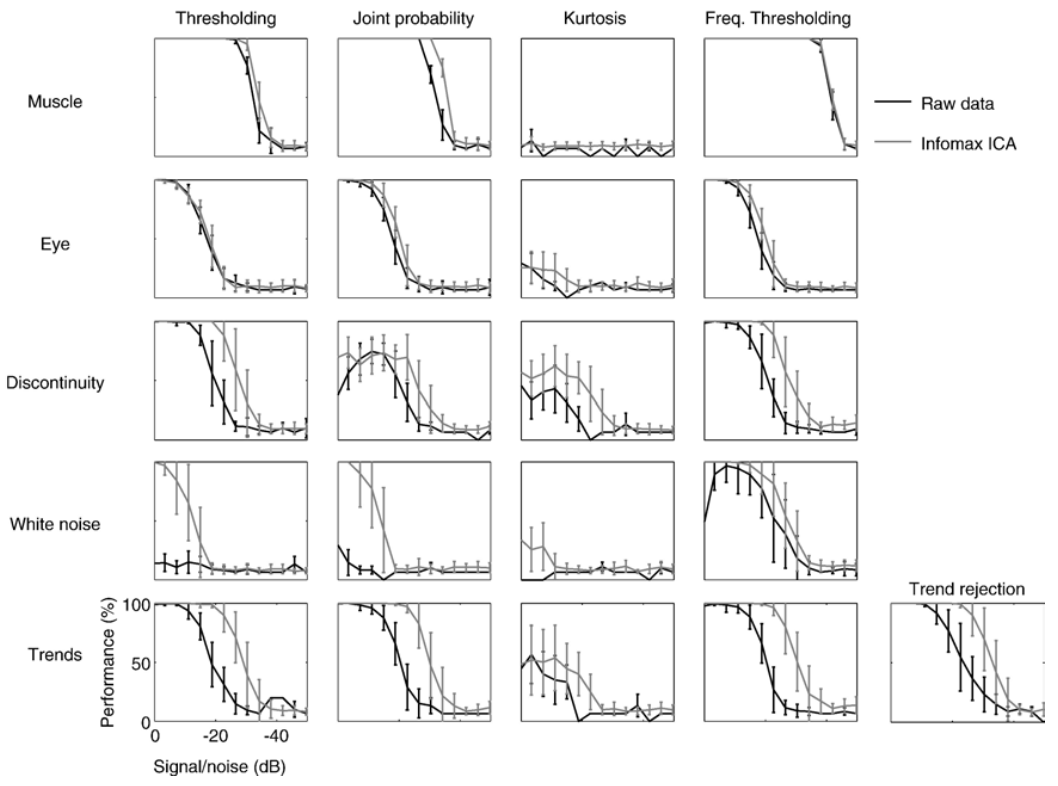
\includegraphics[width=0.9\linewidth,keepaspectratio]{delorme_six}
\caption[Statistical Thresholding of Artifacts]{Classification performance of thresholding approaches based upon the signal to noise ratio of the artifact and the signal.}
\label{fig:delorme_six}
\end{figure}
%%%%%%%%%%%%%%%%%%%

The largest changes in performance were related to the artifacts (discontinuity and white noise) and not the algorithms. This suggested that the algorithm's performance does matter, i.e. Kurtosis performed universally poor, but \ac{ICA} was only able to impact performance when the noise was distinct from the signal. This, of course, is the definition of \ac{ICA}, but highlighted the problem of its use on \ac{EEG} data where waveforms and artifacts presented as seemingly identical signals.

Despite this limitation, these experiments were mostly a success which lead to the development of \ac{FASTER} \cite{Nolan2010} and \ac{ADJUST} \cite{Mognon2011}. These techniques provided universal artifact detection and rejection across multiple types of \ac{EEG} data. \ac{FASTER} relied on a parameter set consisting of variance, Hurst exponent\footnote{The Hurst exponent is a measure of the changes in lag observed from the auto-correlation of pairs of points in a time series.}, amplitude range, and channel deviation over five thresholding levels (channel, epoch, epoch \ac{ICA}, channel-epochs, and channel average). \ac{ADJUST} used spatial and temporal feature extraction to classify and remove artifacts  from \ac{ICA} filtered data. These results again highlighted how different feature sets and algorithms achieved acceptable performance making it hard to know which option is `right'.

%%%%%%%%%%%%%%%%%%%
\begin{table}[ht]
\centering
\caption[FASTER's artifact detection performance]{The sensitivity and specificity at the channel and epoch level for FASTER with respect to different channel configurations.}
\begin{tabular}{l c c c c}
\toprule
Channels & \makecell{Channel\\Sensitivity(\%)} & \makecell{Channel\\Specificity(\%)} & \makecell{Epoch\\Sensitivity(\%)} & \makecell{Epoch\\Specificity(\%)} \\
\midrule
128 & 94.47 & 98.96 & 60.24 & 97.53 \\
64 & 97.02 & 98.48 & 61.83 & 97.54 \\
32 & 5.88 & 96.81 & 58.64 & 97.49 \\
\bottomrule 
\end{tabular}
\label{tab:nolan}
\end{table}
%%%%%%%%%%%%%%%%%%%

\ac{ADJUST} was more complex, but achieved 60\% sensitivity and 97\% specificity, \cref{tab:nolan}, on 2 second channel independent epochs drawn from 47 subjects. \ac{FASTER} was less complex than \ac{ADJUST} and replicated the clinician's 95.2\% artifact detection performance. The most significant aspect of these results were that the testing dataset was built from 10 subjects that were withheld from the 21 subject training dataset.

Artifact detection and correction continues to be an active research topic, but the reliance on \ac{ICA} remained. Mahajan et al.\cite{Mahajan2015} reported exceptional performance using \ac{ICA} on 12 electrodes followed by \ac{mMSE} and Kurtosis and thresholding. Their eye blink detection algorithm reported 90\% sensitivity and 98\% specificity across four subjects.

These statistical approaches to classification are promising, but they are developed on small datasets with simple goals. Adapting them for use on larger datasets with more extensive classifications needs seemed to be beyond their capability. At the very least they showed when \ac{EEG} signals were broken down to their core components it was possible to reliably discriminate among them. This suggested reiterated the idea that it was possible \ac{ML} algorithms to at least match a clinician's performance.

%%%%%%%%%%%%%%%%%%%%%%%%%%%%%%%%%%%%%
\subsubsection{Supervised Algorithms}

Supervised \ac{ML} algorithms build statistical models from datasets with labeled classes. Each class would ideally represent a subset of related data (artifacts, sleep spindles, or \acp{ET}) that the algorithm would learn to distinguish between. Given a diverse feature set, the algorithms build decision surfaces based upon the strongest statistical properties of the features unique to each known class. These decision surfaces allowed classifications to be learned instead of having to infer them directly from the dataset.

These algorithms were setup with the aim of emulating a clinician's classification performance. In doing so, they tied themselves to the performance of those provided the labeled data. This is the main limitation of supervised learning: The algorithms must be shown what to classify making their success dependent on the properties of the training data. If the test contains a new class, the algorithm will struggle to define it and it may go undetected unless additional analyses were undertaken. However, the strength of this approach is that supervised \ac{ML} classification algorithms work extremely well for well known phenomena (artifacts, seizure, and sleep). This has been shown to be true even when such conditions occurred rarely or  were learned from a small number of epochs \cite{Kindermans2014d}. This naturally meant they worked best paired with phenomena in smaller sets of clinically annotated data (\acp{BCI}, emotions, and workload) \acp{EEG}.

The classification of sleep relied on detecting waveforms known as k-complexes and sleep spindles which are unique to a sleeping brain. There is also generalized brain activity specific to the energy bands that accompany each stage of sleep\cite{Silber2007}. Thus each stage of sleep contains a mixture of unique waveforms and shifts in the rhythms, ratios of energy in the \ac{EEG} bands, and waveforms that make it distinct from other brain conditions. Such behavior is most notable in the that dominant ($>$50\%) alpha rhythms where remain indicative of being awake. Stage 1 typically contains a split (50\%\textbackslash50\%) of alpha and delta rhythms. Stage 2 contains sleep spindles and diminished ($<$20\%) delta rhythms. Stage 3 sees a resurgence (20\%-50\%) of delta rhythms. Stage 4 and \ac{REM} sleep are classified by dominant delta rhythms.

These discrete states made the adaptation of supervised \ac{ML} algorithms straightforward. In Schluter et al.\cite{Schluter2012} the stages of sleep were classified with \acp{DT} by bagging\footnote{Bagging, bootstrap aggregating, is a technique employed to reduce the variance of \ac{ML} algorithms. The original data was re-sampled with replacement to produce multiple data sets containing redundant data.} on an array of physiological data\footnote{Sleep studies frequently collect \ac{ECG}, \ac{EEG},\ac{EMG}, and \ac{EOG}. In this work, aside from \ac{EEG} data, \ac{EMG} and \ac{EOG} were used to help classify the sleep stages.}. The classification was performed on 33,542 30 second epochs drawn from 15 subjects, \cref{tab:sleep_conf}. On the whole separating wakefulness, \ac{REM} sleep, and from the stages of sleep was excellent. However, identifying the distinct stages of sleep proved difficult especially for stage 1 and stage 3. These results incorporated data in addition to the \ac{EEG} recordings, suggesting \ac{EEG} alone may not be sufficient for accurate classification.

%%%%%%%%%%%%%%%%%%%
\begin{table}[ht]
\caption[Confusion matrix of sleep stage classification]{Confusion matrix of sleep stage classification covering wakefulness (W), each stage of non-REM sleep (S1,S2,S3,S4) and REM sleep.}
\centering
\begin{tabular}{ l | r r r r r r }
\toprule
& W & S1 & S2 & S3 & S4 & REM \\
\midrule
W 	& 97.0 	& 2.4 	& 0.6 	& 0.1 	& 0.0 	& 0.5 \\
S1 	& 9.1 	& 58.1 	& 20.2 	& 0.8 	& 0.2 	& 11.6 \\
S2 	& 0.5 	& 4.7 	& 91.7 	& 5.5 	& 0.8 	& 0.2 \\
S3 	& 0.0 	& 0.1 	& 20.2 	& 62.8 	& 18.2 	& 0.1 \\
S4 	& 0.1 	& 0.2 	& 1.0 	& 12.6 	& 86.8 	& 0.1 \\
REM 	& 0.7 	& 2.3 	& 3.0 	& 0.1 	& 0.0 	& 96.6 \\
\bottomrule
\end{tabular}
\label{tab:sleep_conf}
\end{table}
%%%%%%%%%%%%%%%%%%%

Radha et al. \cite{Radha2014} used different algorithms to classifying the stages of sleep, but produced similar results to that of Schluter et al. Their data consisted of 30s epochs of 34 features drawn from 10 health subjects. They compared two supervised algorithms, \ac{RF} and \ac{SVM}, ability to classify the epochs into \ac{REM} sleep and the 3 stages of non-\ac{REM} sleep (N1,N2,N3). By using supervised algorithms it was necessary to have a clinician provide labeled training data. However, this also allowed a $\kappa$ statistic to be associated with each algorithm's performance relative to the clinician, \cref{tab:radha}. Prior to classification the feature set was optimized for the differential montage channel (F4-A1), an epoch duration of 30s, and only 20 of the original 34 features.

%%%%%%%%%%%%%%%%%%%
\begin{table}[ht]
\caption[Single EEG Channel Sleep Scoring]{Precision and recall of SVM and RF classification using a single EEG channel for sleep stage classification. In this study non-REM sleep is broken into only three stages (N1, N2, N3) making it difficult to compare to the standard four non-REM stages of sleep shown in \cref{tab:sleep_conf}.}
\centering
\begin{tabular}{c | c c c c c c}
\toprule
\makecell{Sleep\\Stage} & \makecell{SVM 1vA\\Precision} & \makecell{SVM 1vA\\Recall} & \makecell{SVM 1v1\\Precision} & \makecell{SVM 1v1\\Recall} & \makecell{RF\\Precision} & \makecell{RF\\Recall}\\
\midrule
W 		& 0.86 & 0.51 & 0.75 & 0.71 & 0.78 & 0.73 \\
N1		& 0.00 & 0.00 & 0.18 & 0.00 & 0.52 & 0.31 \\
N2		& 0.86 & 0.83 & 0.85 & 0.88 & 0.85 & 0.91 \\
N3		& 0.32 & 0.70 & 0.82 & 0.70 & 0.83 & 0.73 \\
REM 	& 0.56 & 0.55 & 0.58 & 0.79 & 0.69 & 0.70 \\
\midrule
Accuracy & \multicolumn{2}{c}{0.69} & \multicolumn{2}{c}{0.77} & \multicolumn{2}{c}{0.80} \\
$\kappa$ & \multicolumn{2}{c}{0.46} & \multicolumn{2}{c}{0.61} & \multicolumn{2}{c}{0.66} \\
\bottomrule
\end{tabular}
\label{tab:radha}
\end{table}
%%%%%%%%%%%%%%%%%%%

These results were comparable, \cref{tab:sleep_conf}, to Schluter et al., which was a study that used far more data. The moderate to substantial $\kappa$ statistics suggested the algorithms performed as well as a clinician would have given the previously reported inter-rater agreements. However, it was possible that the feature optimization drove this performance. Sleep states were not a unique phenomena and they tended to represent major changes in brain activity, the necessity of channel and feature optimization suggests this algorithm/feature combination was only able to find the strongest indicator of sleep and may be missing out on the nuances of individual sleep stages.

Similar to sleep, seizures had frequently been categorized into distinct stages: \emph{normal} indicative of a normal healthy state, \emph{pre-ictal} indicative of a build up to a seizure, \emph{ictal} indicative of an active seizure \cite{Acharya2012}, and \emph{post-ictal} indicative of the time following a seizure \cite{Chu2017}. Accurate detection of these stages, specifically pre-ictal, could help improve the diagnosis and treatment of epilepsy \cite{Ramgopal2014}. Seizure classification was always a primary research focus of automated algorithms because of number of people affected by them\cite{Ramgopal2014}. Effort has been continually applied to improve the classification of seizures which tended to focused on developing better features than the \ac{FFT} based frequency band powers \cite{Wulsin2011,Bajaj2012,Chu2017} and improving algorithms \cite{Acharya2012,Ghosh-Dastidar2007,Subasi2005}. These efforts were predicated on, and thus limited by, the availability of annotated data and the quality of the annotations.

Wulsin et al.\cite{Wulsin2011} used raw data and diverse feature subsets derived from a stock listing of features \footnote{area, normalized decay, frequency band power, line length, mean energy, average peak/valley amplitude, normalized peak number, peak variation, root mean square, wavelet energy, and zero crossings} to compare seizure detection as a function of algorithms and features. Despite efforts to find a suitable feature subset, the strongest classification occurred when using the raw data as the input features. In addition to the feature analysis, four classification algorithms (\acp{DT}, \acp{SVM}, \acp{KNN}, and \acp{DBN}) were evaluated with \acp{SVM} producing the best classifications, \cref{fig:wulsin2011_f1}.

%%%%%%%%%%%%%%%%%%%
\begin{figure}[ht]
\centering
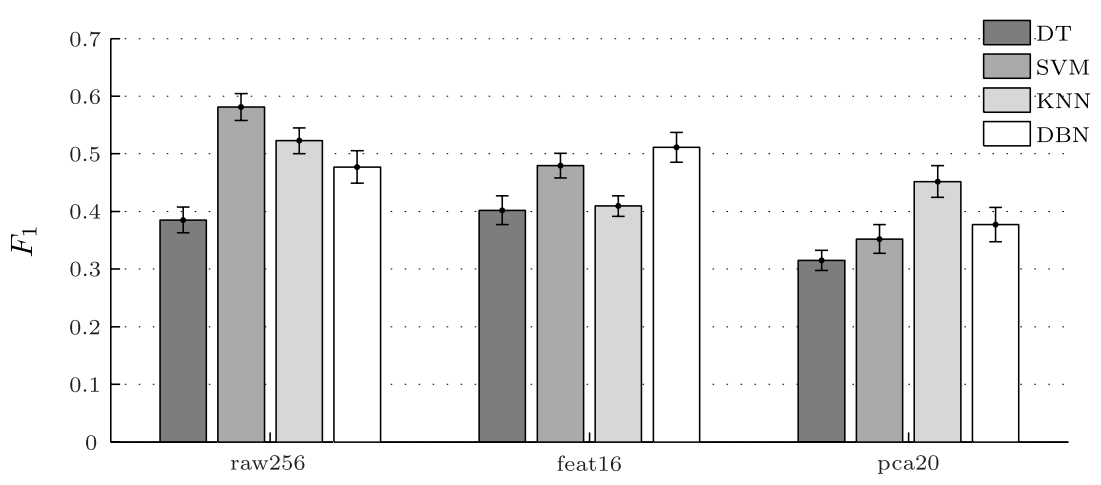
\includegraphics[width=0.75\linewidth,keepaspectratio]{wulsin2011_f1}
\caption[F1 Performance of Four Supervised Algorithms]{Wulsin et al. evaluate algorithm peformance based upon the $F_{1}$ measure, where $F_{1}=2*(sensitivity*precision)/(sensitivity+precision)$. The results are presented to compare the algorithms and feature sets against each other. The feature sets are comprised of: \textit{raw256} represents the raw waveform data, \textit{feat16} are the hand selected 16 features, and \textit{pca20} are the 20 features chosen by \ac{PCA}. }
\label{fig:wulsin2011_f1}
\end{figure}
%%%%%%%%%%%%%%%%%%%

Bajaj et al.\cite{Bajaj2012} used \ac{EMD}\footnote{A detailed review of \ac{EMD} is omitted, but if interested the work of Huang et al.\cite{Huang1998} introduced technique and its applications.} features as inputs for a \ac{LSSVM} driven seizure classifier. The data was sourced from 100 23.6s channel epochs drawn from 5 subjects. \ac{EMD} separated the nonlinear and non-stationary components of the \acp{EEG} into \acp{IMF}. The two dominant \acp{IMF}, amplitude modulation and frequency modulation, produced a peak sensitivity and specificity of 100\% while averaging 94\% sensitivity and specificity over the dataset by using a common supervised \ac{ML} algorithm in \acp{SVM}. As the classifier was not knew, the success of this work was likely driven by the use of \ac{EMD} features or qualities of the 5 subject dataset. This was a recurrent problem with \ac{EEG} algorithm development of unique datasets and unique features obscuring the cause of classification improvement.

The alternative to diverse features and datasets was to test  range of algorithms. This is what Acharya et al.\cite{Acharya2012} did by focusing on six supervised \ac{ML} algorithms: \ac{FSC}, \ac{SVM}, \ac{KNN}, \ac{PNN}, \ac{DT}, and \ac{NBC}, and one unsupervised \ac{ML} algorithm: \ac{GMM}. This was a better approach than Bajaj et al.'s as it provides multiple reference points on a constrained dataset. These six algorithms used four different types of entropy calculations as features: \ac{APEN}\cite{Pincus1991}, \ac{SAMPEN}\cite{Richman2000}, and S1 entropy and S2 entropy\cite{Nikias1993}. Distinct epochs were drawn from 5 healthy and 5 epilepsy subjects that produced 200 healthy, 200 pre-ictal, and 100 ictal artifact free single channel 23.6 second epochs.

%%%%%%%%%%%%%%%%%%%
\begin{table}[ht]
\caption[Classification accuracy of entropy based feature sets]{Classification accuracy of entropy based feature sets for various classifiers.}
\centering
\begin{tabular}{ l c c c }
\toprule
Algorithm & Accuracy (\%) & Sensitivity (\%) & Specificity (\%) \\ \midrule
FSC 	& 98.1 & 99.4 & 100\\
SVM 	& 95.9 & 97.2 & 100\\
KNN 	& 93.0 & 97.8 & 97.8\\
PNN 	& 93.0 & 97.8 & 97.8\\
DT 	& 88.5 & 98.3 & 91.1\\
GMM 	& 95.9 & 98.3 & 95.6\\
NBC 	& 88.1 & 94.4 & 97.8\\
\bottomrule
\end{tabular}
\label{tab:acharya}
\end{table}
%%%%%%%%%%%%%%%%%%%

The sensitivity and specificity the algorithms were similar, \cref{tab:acharya}, but the best accuracy was achieved by the \ac{FSC} classifier. The separability of the trained seizure states, \cref{tab:acharyaFeats}, produced a $p$-value less than 0.0001 for each entropy. However, it was hard to assess the strength of the individual algorithms given the small size of the dataset and the natural discrimination strength of the features. The strong performance across all the algorithms suggested the results were driven by the features, but the dataset was, again, too small to have known for certain. 

%%%%%%%%%%%%%%%%%%%
\begin{table}[ht]
\caption[Entropy levels based upon seizure state]{The level of entropy for each feature with respect to the classified seizure state.}
\centering
\begin{tabular}{ l l l l }
\toprule
Class & Normal & Pre-ictal & Epileptic \\
\midrule
ApEn 		& $2.2734\pm3.320\times10^{-2}$ 	& $1.8650\pm0.331$ & $1.9325\pm0.215$ \\
SampEn 		& $1.3130\pm0.120$					& $0.99332\pm0.189$ & $0.92628\pm0.139$ \\
S1 			& $0.57012\pm7.120\times10^{-2}$	& $0.47208\pm6.149\times10^{-2}$ & $0.48325\pm1.55$ \\
S2 			& $0.76827\pm3.125\times10^{-2}$	& $0.68072\pm3.790\times10^{-2}$ & $0.73184\pm4.555\times10^{-2}$\\ 
\bottomrule
\end{tabular}
\label{tab:acharyaFeats}
\end{table}
%%%%%%%%%%%%%%%%%%%

Ghosh-Dastidar et al. \cite{Ghosh-Dastidar2007} benchmarked a novel wavelet-chaos-neural network \ac{LMBPNN} classifier against the same data as Acharya et al. They picked features (standard deviation, correlation dimension, and largest Lyapunov exponent) that were specific to each frequency band and grouped them together into various band specific sets. The epochs were evaluated by supervised techniques (\ac{RBFNN} and \ac{LMBPNN}), an unsupervised technique ($k$-means clustering), and statistical discriminant techniques (\ac{QDA} and \ac{LDA} using Euclidean and Mahalanobis distance metrics).

The various combination of band-specific features sets were used to resolve an optimal set for the classifiers. These tests provided an exhaustive analysis of the relationship between algorithm and feature set performance, which was frequently lacking in other research. However, the best performance resulted when using a mixed-band feature set. The impact of feature set on the performance of \ac{LMBPNN} is seen in \cref{fig:ghoshLMBPNN}.

%%%%%%%%%%%%%%%%%%%
\begin{figure}
\centering
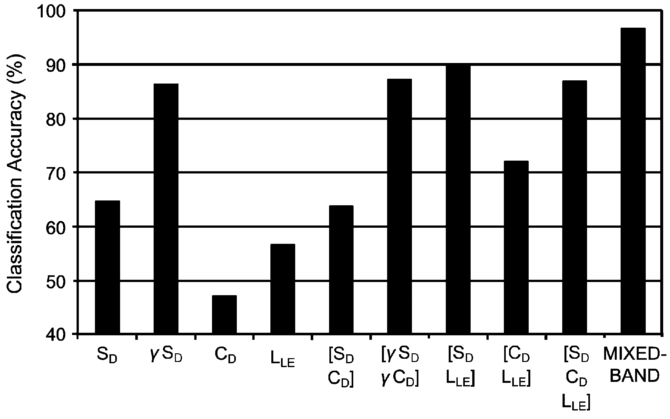
\includegraphics[width=0.75\linewidth,keepaspectratio]{ghoshLMBPNNfeat}
\caption[Impact of features on LMBPNN classification]{When iterating over the available feature sets, the performance of \ac{LMBPNN} responds differently for each combination. The Greek letters indicate the band specific features ($S_{D}$ is standard deviation, $C_{D}$ is correlation dimension, and $L_{LE}$ is Lyapunov exponent). The mixed-band feature set uses the band independent $S_{D}$ and $C_{D}$ with $\alpha S_{D} C_{D} L_{LE}$, $\beta S_{D} C_{D}$ and $\gamma S_{D} C_{D}$.}
\label{fig:ghoshLMBPNN}
\end{figure}
%%%%%%%%%%%%%%%%%%%

The classification performances were similar so only the maximum accuracy was reported in \cref{tab:ghosh} and even these cover a wide range. Overall, the proposed \ac{LMBPNN} provided the strongest peak performance, but it relied on a large mixed-band feature set. This suggested that the features were the driving force of classification, and yet only some of the algorithms were able to adequately used them. Again, the difficulty in improving performance appeared to stem from being able to model the phenomena in a meaningful way for the chosen classifiers.

%%%%%%%%%%%%%%%%%%%
\begin{table}[ht]
\caption[Classification accuracy of single and mixed band feature sets]{The table reports the maximum accuracy achieved by each algorithm given on a single or (*) mixed-band feature set.}
\centering
\begin{tabular}{ c c }
\toprule
Algorithm & Maximum Accuracy (\%) \\
\midrule
$k$-means & 59.3 \\
LDA w/ Euclidean & 79.6 \\
LDA w/ Mahalanobis & 84.8 \\
QDA & 85.5 \\
RBFNN & 76.5 \\
LMBPNN & 89.9 \\
QDA* & 93.8 \\
LMBPNN* & 96.7 \\
\bottomrule
\end{tabular}
\label{tab:ghosh}
\end{table}
%%%%%%%%%%%%%%%%%%%

%%%%%%%%%%%%%%%%%%%%%%%%%%%%%%%%%%%%%%%
\subsubsection{Unsupervised Algorithms}

Unsupervised \ac{ML} algorithms differed from supervised \ac{ML} algorithms in that they do not require labeled data. This has made them a historically useful as starting point when knowledge of a domain was limited. Their decision surfaces were created directly through the data which removed any bias present in the labeling, but traded it for bias in the datasts. This also meant unsupervised approaches worked best when operating on datasets with enough data to represent each class of interest. Thus without an equitable distribution of data, classes may be ignored or poorly modeled leading to weak classification performance.

Given the need for large and diverse datasets and improvement to supervised classification techniques, the use of unsupervised classification of \ac{EEG} recordings has diminished. However, unsupervised algorithms endured given their ease of use and ability to produce benchmarks for their supervised counterparts. Acharya et al.\cite{Acharya2012} showed \ac{GMM} produced competitive accuracy and sensitivity, but not specificity to their tested supervised methods in \cref{tab:acharya}. Alternatively, there were cases where it peformed much worse such as Ghosh-Dastidar et al.'s \cite{Ghosh-Dastidar2007} $k$-means clustering of \cref{tab:ghosh}. As unsupervised algorithms relied on the dataset more than supervised techniques, such contrasting performances were common in the \ac{EEG} literature.

Gabor et al.\cite{Gabor1996} tested a single unsupervised algorithm, a \ac{SOM}\footnote{A detailed review of \acp{SOM} was omitted, but if interested the work of Kohonen\cite{Kohonen1990} formalized the implementation. This technique attempts to mimic the structure of the brain by parsing the data in an unsupervised fashion to create a flat, two dimensional, map linking elements of the data together.} \ac{NN}, for seizure detection on 24 recordings from 22 subjects. The algorithm was trained to classify seizures from features produced by a wavelet transform using 4s epochs built from the 10 channels of each recording. A separate feature set using 8s epochs was used, but the duration was found to be too long as it masked out shorter seizures.

In total 62 seizures were captured from the 24 recordings of which the algorithm detected 56 (90\%). The average false positives per hour (0.71) produced more false positives than true positives given the average recording duration of 22.02 hours. As discussed previously, unsupervised techniques are sensitive to the distribution of the training data which manifested in this case as poor false alarm rates. In addition, the age range ($<$1 to 43 years old), small training set (5 of the 24 recordings), and epoch duration were all factors working against the algorithm.

Not all unsupervised algorithms focus on classifying the data, as some are deployed for dimensionality reduction. One such approach was the use of of unsupervised \ac{LDA} in areas where clinicians' skills were weaker such as \ac{BCI} \cite{Vidaurre2011}. \ac{LDA} is within the realm of \ac{FA}, as are \ac{ICA} and \ac{PCA}.  A detailed review of \ac{FA} techniques is given in Section \ref{sec:FA} and what follows now touches on their use in \ac{EEG} applications.

Vidaurre et al. \cite{Vidaurre2011} used three flavors of \ac{LDA} to enhance \ac{BCI} performance over four datasets\footnote{The first dataset was comprised of 19 sessions recorded from 10 subjects performing motor imagery tasks. The second dataset consisted of 80 subjects performing 75 motor imagery trials with calibration. The third dataset involved 7 quadriplegics attempting to move use a \ac{BCI} mouse. The final dataset was a repeat of the second dataset without any calibration for the users.}. The experiments focused on developing an unsupervised solution to transitioning between training and feedback sessions of \ac{BCI} tasks. Each version of \ac{LDA} focused on a different aspect of the features: LDA-I, targeted changes in the \ac{PMEAN} between the features of the training and feedback data, LDA-II incorporated updates to the covariance matrix with \ac{PMEAN}, and LDA-III scaled the mean and covariance  using \acp{CSP}. These techniques were compared against a supervised version of \ac{LDA} to determine the strength of the unsupervised techniques.

%%%%%%%%%%%%%%%%%%%
\begin{figure}[ht]
\centering
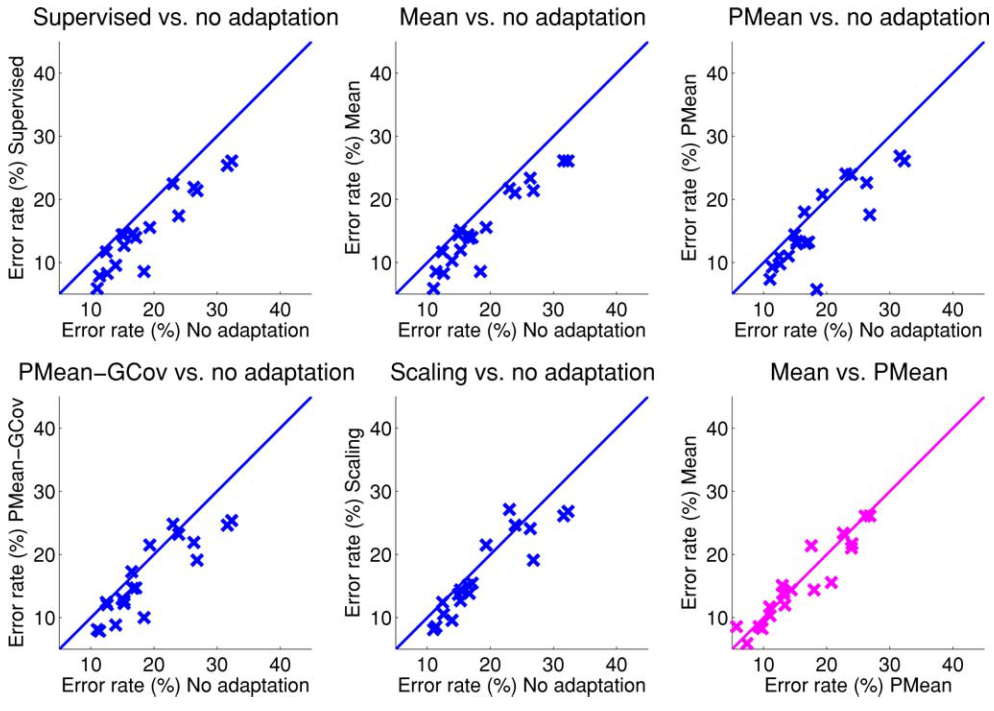
\includegraphics[width=0.75\linewidth,keepaspectratio]{vidaurre2011_error}
\caption[BCI Calibration Error]{The comparative error rates between the supervised and unsupervised adaptation techniques through changes in the error rate. The pink plot shows the difference between a labeled, mean, and unlabeled, \ac{PMEAN}, classification.}
\label{fig:vidaurre2011_error}
\end{figure}
%%%%%%%%%%%%%%%%%%%

Unsupervised techniques main strength resides in their simplicity when compared to ever advancing supervised techniques. Their evaluation was frequently used to evaluate the performance gain versus increased complexity and requirements. This made head to head comparisons, \cref{fig:vidaurre2011_error}, critical to development of both type of algorithm. Using the first dataset, the supervised algorithms slightly out performed the unsupervised algorithms. On the second, larger, dataset the \ac{PMEAN} based algorithms met or exceeded the performance of the state of the art supervised approaches during feedback. The unsupervised technique exhibited robustness as a class was removed from \ac{BCI} feedback and outperformed the supervised algorithm in \cref{fig:vidaurre2011_feedback}. These results were important because clinicians seldom label \ac{BCI} datasets and it showed the trade off between supervised and unsupervised may not be that advantageous. This was especially true in this instance as \ac{BCI} recording sessions were rarely annotated by clinicians, but often as dynamic as seizure or sleep sessions.

%%%%%%%%%%%%%%%%%%%
\begin{figure}[ht]
\centering
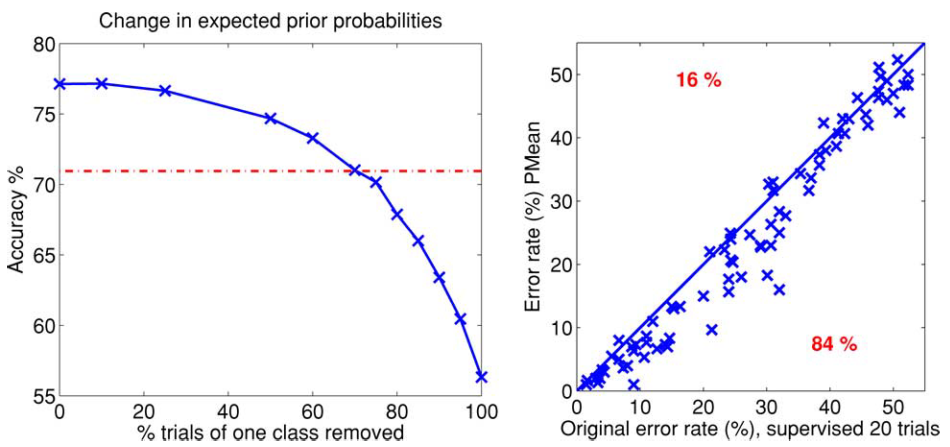
\includegraphics[width=0.75\linewidth,keepaspectratio]{vidaurre2011_feedback}
\caption[BCI Feedback Error]{Performance on feedback data after training for supervised adaptation and unsupervised \ac{PMEAN} adaptation. The (left) impact of removing one class from the feedback dataset for the supervised algorithm (red line) and unsupervised algorithm (blue line). The (right) error rate between the two algorithms during the online feedback experiments.}
\label{fig:vidaurre2011_feedback}
\end{figure}
%%%%%%%%%%%%%%%%%%%

%%%%%%%%%%%%%%%%%%%%%%%%%%%%%%%%%%%%
\subsection{Bio-metric Applications}

The use of \ac{EEG} recordings as a means of bio-metric identification was not dominant area of research, but has begun to rapidly advance \cite{Delpozo-Banos2015}. Initial efforts focused on being able to discriminate \ac{EEG} behavior between individuals and between different brain conditions \cite{VanDis1979}. This work did not have discrete waveforms to find or frequency ratios to calculate, but instead relied on direct comparison between subjects. Stassen \cite{Stassen1980} developed computerized methods, borrowed from speech recognition, to recognize normal and schizophrenic individuals based on their \ac{EEG} spectral pattern. The style of this approach, finding dominant properties in subject epochs, remained in use \cite{DelPozo-Banos2014a} and was the best corollary to the research proposed in this dissertation.

Advancement of \acp{EEG} as a bio-metric tool focused on the statistical properties of each subject \cite{Delpozo-Banos2015}. This detached it from the dominant research trends that were reliant on clinical annotations \cite{Marcel2007a}. This made bio-metric applications open-ended as they do not, and in most cases cannot, rely on previously developed feature sets or decision surfaces built from clinical annotations. Researchers were therefore on their own to find features and testing protocols leading to a variety of approaches not seen elsewhere \cite{VanBeijsterveldt2002,Rocca2013,Rodrigues2016,Ruiz-blondet2016,Nguyen2013}.

The initial efforts by VanDis et al.\cite{VanDis1979} and Stassen \cite{Stassen1980} focused on subjects at rest with eyes closed and open. Similar experiments contiuned to be carried out \cite{Rocca2012,Rocca2014,Rocca2013} but with their aims updated to optimize the accuracy and speed of subject verification as a function of features and channels. Active state recordings, when subjects performed mental tasks, such as imagined hand movements \cite{Fraschini2015,Marcel2007a}, imagined speaking syllables \cite{Brigham2010}, or reading text\cite{Gui2015} underwent similar channel and feature optimization testing.

Active and resting based data analysis suggested that the qualities of subject authentication and identification existed regardless of brain state. Other works went as far as suggesting a genetic basis underlies this separability \cite{Begleiter2006,DeGennaro2008}. While interesting, the genetics of brain uniqueness expanded beyond the scope of this work. However, by focusing on the techniques and results of active and resting based data studies comparisons could likely be drawn between the structured waveform based annotations of artifacts, seizures, and sleep.

%%%%%%%%%%%%%%%%%%%%%%%%%%%%%%%%%%
\subsubsection{Resting Recordings}

The work of La Rocca et al.\cite{Rocca2012,Rocca2014,Rocca2013} focused on developing a novel set spatial and temporal patterns as features to improve subject recognition. Brigham et al.\cite{Brigham2010} used data with imagined activities to test applications of subject identification during mental tasks. These studies represent the adaptation of techniques the worked for other \ac{EEG} classification tasks, spatial and temporal patterns for \ac{BCI} and mental tasks for attention/focus/workload performance and \acp{ERP}.

In \cite{Rocca2012} electrode sets of 2, 3, and 5 from the 56 recorded channels were used to find a lower-bound on the number of required channels. The approach used autoregressive stoichastic modeling and polynomial regression to match 3 second epochs broken into features through the 6 standard \ac{EEG} bands. Classification performance varied as a function of electrode set and the \ac{EEG} band used. Increasing electrodes trended with an improvement in classification performance. However, regardless of the number of electrodes the alpha band provided the strongest classification accuracy. Performance peaked at 98\% classification accuracy when using the alpha, beta, delta, and gamma bands for 5 channel sets. The best single band performance (83\%) was seen using only the alpha band across 5 channels.

They followed up this work with `bump' modeling to reduce the amount of data from the 10-20 layout into a parametric model \cite{Rocca2013}. These bumps were filters that enabling sparse encoding. This generated vectors  to control the mapping/weights of the bumps scale the features of the data. These vectors were then classified with \ac{LDA} based upon features generated from groups of three channels drawn from the six standard \ac{EEG} bands. The training and testing sets were curated to provide overlapping frames, \emph{jointed}, and without overlapping frames, \emph{disjointed}. This distinction highlighted the impact of frame overlapping with the beta band producing a classification accuracy of 95\% for jointed and 74\% for disjointed. The alpha band resulted in similar classification accuracy with 96\% for jointed and 67\% for disjointed. In all bands the jointed feature sets outperformed their disjointed counterparts.

Their final work focused on spatial patterns generated from 1s \acp{PSD} epochs from different regions of the brain \cite{Rocca2014}. This deviated from their earlier attempts at reducing the amount of data through feature and individual channel reduction. Instead it grouped channels together to develop a statistical approach to subject verification using the \ac{PNET} dataset. Classification was carried out by building Gaussian mixtures based upon the distributions of the \acp{PSD}. These mixtures were evaluated via a \ac{MD} classifier to determine likelihood of similarity between subjects. Using the results for each region of the brain, classification accuracy reached 100\% for identifying subjects.

%%%%%%%%%%%%%%%%%%%%%%%%%%%%%%%%%
\subsubsection{Active Recordings}

In Marcel et al.\cite{Marcel2007a} a nine subject dataset was classified based upon their brain activity during three mental tasks. These tasks required the subjects to imagine carrying out prescribed actions: moving their left hand, moving their right hand, and speaking words with a common leading letter. The feature set was built from 0.5s 50\% overlapping epochs of \acp{PSD}. These \acp{PSD} were spatial filtered over the 10-20 electrode configuration with a surface Laplacian function. The features were given to a \acp{GMM} which produced baseline models for subject verification. Evaluation scores were reported as \ac{HTER} generated from the \ac{FAR} and \ac{FRR}.
\begin{gather}
HTER = \frac{FAR + FRR}{2}
\end{gather}
The results, \cref{tbl:marcel}, of the left and right hand authentication of the subjects suggested performance was dependent on the number of Gaussian mixtures used in the modeling process. This experiment used a large datasets which was collected from the subjects over a three day period. Results using smaller subsets of the dataset showed the imaging word task authentication lagged compared to that of the hand tasks.

%%%%%%%%%%%%%%%%%%%
\begin{table}[ht]
\centering
\caption[Imagined Activity HTER]{The FAR, FRR, and HTER of imagined hand tasks as a function of Gaussian mixtures for Marcel et al.'s experiments.}
\begin{tabular}{|c|c| r r r|}
								\hline
\multicolumn{1}{|l|}{Mental Task} 	& Num. Gaussians 	& FAR 	& FRR 	& HTER \\
								\hline
\multirow{4}{*}{Left} 				& 4 				& 18.6 	& 32.3 	& 25.4 \\
                           			& 8 				& 23.8 	& 25.15 	& 24.5 \\
                            		& 16 			& 19.3 	& 19.65 	& 19.5 \\
                               		& 32 			& 13.7 	& 24.9 	& \textbf{19.3} \\
                               		\hline
\multirow{4}{*}{Right} 			& 4 				& 18.4 	& 40.5 	& 29.4 \\
                               		& 8 				& 20.6 	& 29.5 	& 25.0 \\
                                	& 16 			& 15.0 	& 23.6 	& \textbf{19.3} \\
                              		& 32 			& 13.0 	& 30.15 	& 21.6 \\
                                	\hline
\end{tabular}
\label{tbl:marcel}
\end{table}
%%%%%%%%%%%%%%%%%%%

In Fraschini et al.\cite{Fraschini2015} phase synchronization was tested as a feature set for identifying subjects. The dataset used the 109 \ac{PNET} subjects' resting eyes closed and resting eyes trials. The features were generated from the standard \ac{EEG} frequency bands and segmented into 12s non-overlapping epochs. Finding the \ac{PLI} relationship between all the channels of an epoch produces distinct mappings between subjects. These topologies were reduced via \ac{EC} to produce a feature vector for each epoch. The \ac{ED} between each feature vector was the decision surface used to assert the similarity between the subjects for each frequency band.

%%%%%%%%%%%%%%%%%%%
\begin{table}[ht]
\centering
\caption{EER of phase synchronization based subject verification}
\begin{tabular}{l r r}
\toprule
Band & REO EER (\%) & REC EER (\%) \\ \midrule
Gamma & 4.4 & 6.5 \\
Beta & 10.2 & 16.9 \\
\bottomrule
\end{tabular}
\label{tbl:fraschini}
\end{table}
%%%%%%%%%%%%%%%%%%%

Brigham et al.\cite{Brigham2010} tested a similar subject identification protocol using two unique datasets. One source of data came from \acp{VEP} in 120 alcoholic and non-alcoholic subjects. The other ws sourced from 6 subjects uttering two syllables, /ba/ and /ku/. Artifacts were removed from each set and processed into \acp{PSD} of their respective trial lengths, 1s for the \ac{VEP} and 10 seconds for the syllables. Using \acp{SVM} and \acp{KNN} the classification accuracy of each algorithm was averaged from 4-fold cross-validation. After artifact removal the \ac{VEP} data set contained 9,596 trials for the 120 subjects and 3,787 trials for the 6 syllable subjects.

On the \ac{VEP} dataset the \ac{SVM} achieved 98\% accuracy and \ac{KNN} achieved 93\% accuracy, both had a 95\% confidence interval. The syllable dataset achieved higher accuracy, 99\% with \ac{SVM} and 98\% with \ac{NN} with both, again, at a 95\% confidence interval. The strong performance across both datasets indicated the techniques and feature sets worked well on a fundamental level. However, the diminutive number of syllable subjects was not compelling and should have likely be run with more subjects.

In Gui et al.\cite{Gui2015} a more contemporary \ac{ML} technique, \ac{ANN} using feed-forward, back-propagation, and multiplayer perceptron, was used to identify subjects. Their dataset consists of the 6 mid-line channels \{Fpz, Cz, Pz, O1, O2, and Oz\} of 32 subjects undergoing \acp{VEP}. The channels were bandpass filtered, 0Hz to 60Hz, before \ac{WPD} produces the final three features of mean, variance, and entropy for each 1.1 second epoch. Four experiments are carried out, but only two were of interest in subject classification: (S1) finding a single subject from the set of 32 and (S2) matching all 32 subjects against each other simultaneously. The other experiments consisted of a one versus all classification (S3) and separating small groups of subjects from each other (S4). For S1 the highest accuracy of 10\% occurred with 5 neurons and the worst accuracy of 5\% occurred with 10 neurons. S2 produced better results with a highest accuracy of 94\% with 45 neurons and a worst accuracy of 70\% with 30 neurons.

Here the fundamental issues of \ac{ML} were exposed in terms of dataset source, pre-processing, feature selection, algorithm, and classification task. Across the range of experiments presented nearly every single one used different data or different features or different algorithms. The result was a lack of comparison points from which to drawn definitive conclusions about \acp{EEG} data and features or their classification. While many of these experiments produced acceptable results, little was gained and many were often confirming ideas already well documented instead of expanding the knowledge base.

%%%%%%%%%%%%%%%%%%%%%%%%%%
\section{Identity Vectors}

At the center of this dissertation was the introduction of \acp{IV} to the \ac{EEG} classification community. \acp{IV} are mathematical models that were designed to reduce the dimensionality of \acp{UBM} \cite{Kenny2008b}. \acp{UBM} served to reduce a dataset of $f$-dimensional feature samples into $C$ mixtures of $f$-dimensional \acp{GMM}. Following this, \acp{IV} can then be created by enrolling distinct samples into a modeling process involving the \ac{UBM} and a \ac{TVM}. The \ac{TVM} is generated from the enrollment samples and served to constrain the contributions of each mixture within the \ac{UBM}. Finally, those \acp{IV} were evaluated against testing \acp{IV}, built from testing samples and the same \ac{TVM} used to produce the enrollment \acp{IV}. This evaluation resolve the distance in the $l$-dimensional distance between them.

As the technique is entirely data dependent, it could be altered to measure similarities between epochs, channels, individuals, or groups of individuals. \acp{IV} were developed originally as an extension of a speech processing method called \ac{JFA} which split utterances into separate models for speaker, channel, and context \cite{Kenny2007b}. In contrast, \acp{IV} collapse those three models into just one.

The principal \ac{IV} equation is 
\begin{equation}
M\approx m+Tw
\label{eq-iVec_raw}
\end{equation}
where $M$ is the feature space of the data, $m$ is the \ac{UBM}, $T$ is the \ac{TVM} and $w$ is the \ac{IV} itself. The specific data used to build the \ac{UBM} $m$ is referred to as the training data. Once $m$ and $T$ have been defined, they can be used in concert with alternate enrollment targets of size $S$ and testing data sets $M$ to create data-specific \acp{IV}, $w$.

%%%%%%%%%%%%%%%%%%%
\begin{figure}[ht]
\centering
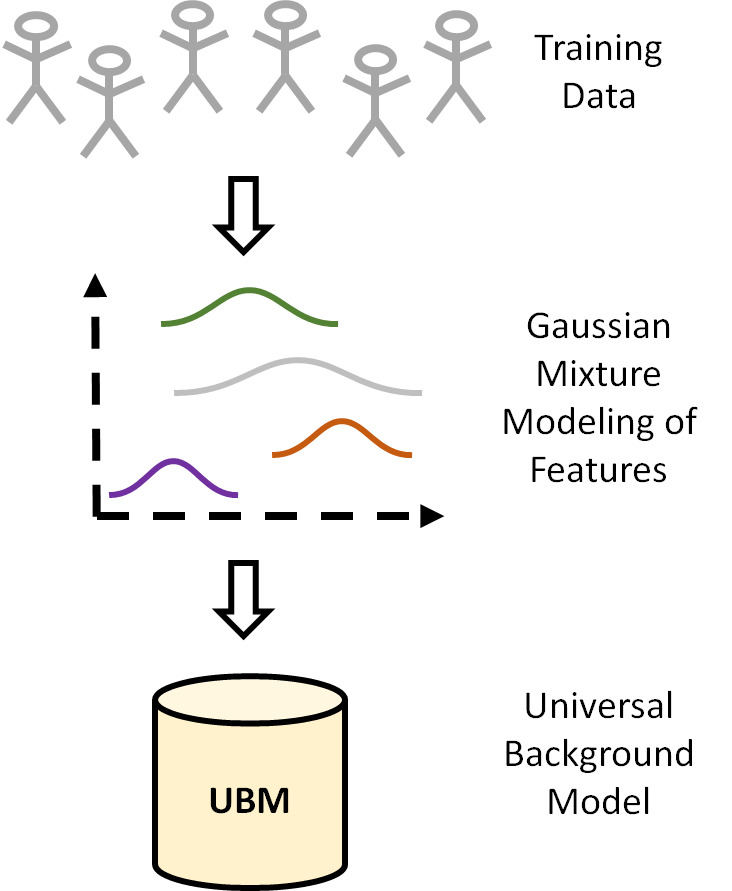
\includegraphics[height=0.5\linewidth,keepaspectratio]{figure1}
\caption[UBM Development]{Training data was used to construct $C$ independent Gaussian mixtures over the $f$ dimensional feature space. This transformed the training data into $C$ mixtures each with $f$ means and variances. Taken as a whole these $c$ mixtures were the \ac{UBM} in addition to a mixture weight parameter. Ultimately this $c$ mixture \ac{UBM} served as the basis for developing a \ac{TVM} and the associated \acp{IV}.}
\label{fig:ubm}
\end{figure}
%%%%%%%%%%%%%%%%%%%

A typical \ac{IV} use case might involve determining whether an \ac{EEG} from a new patient should be diagnosed as epilepsy. First, a large randomized collection of training data drawn from a diverse set of subjects would be used to build a \ac{UBM}, \cref{fig:ubm}. Then, sub-populations of data from known healthy and epileptic patients would be used to construct an enrollment dataset. This enrollment dataset would be used to resolve a \ac{TVM} and produced enrollment \acp{IV} related to the enrollment subjects.

Finally, the new patient's data would be used with the \ac{TVM} to construct their \acp{IV}. Then evaluations between the enrollment and target \acp{IV} would inform which population they were more likely to match with, \cref{fig:iVector}. Depending on the choice of enrollment and test data, \acp{IV} can automatically search for across channels, times, medical conditions, medications, and even entire subjects.

%%%%%%%%%%%%%%%%%%%
\begin{figure}[ht]
\centering
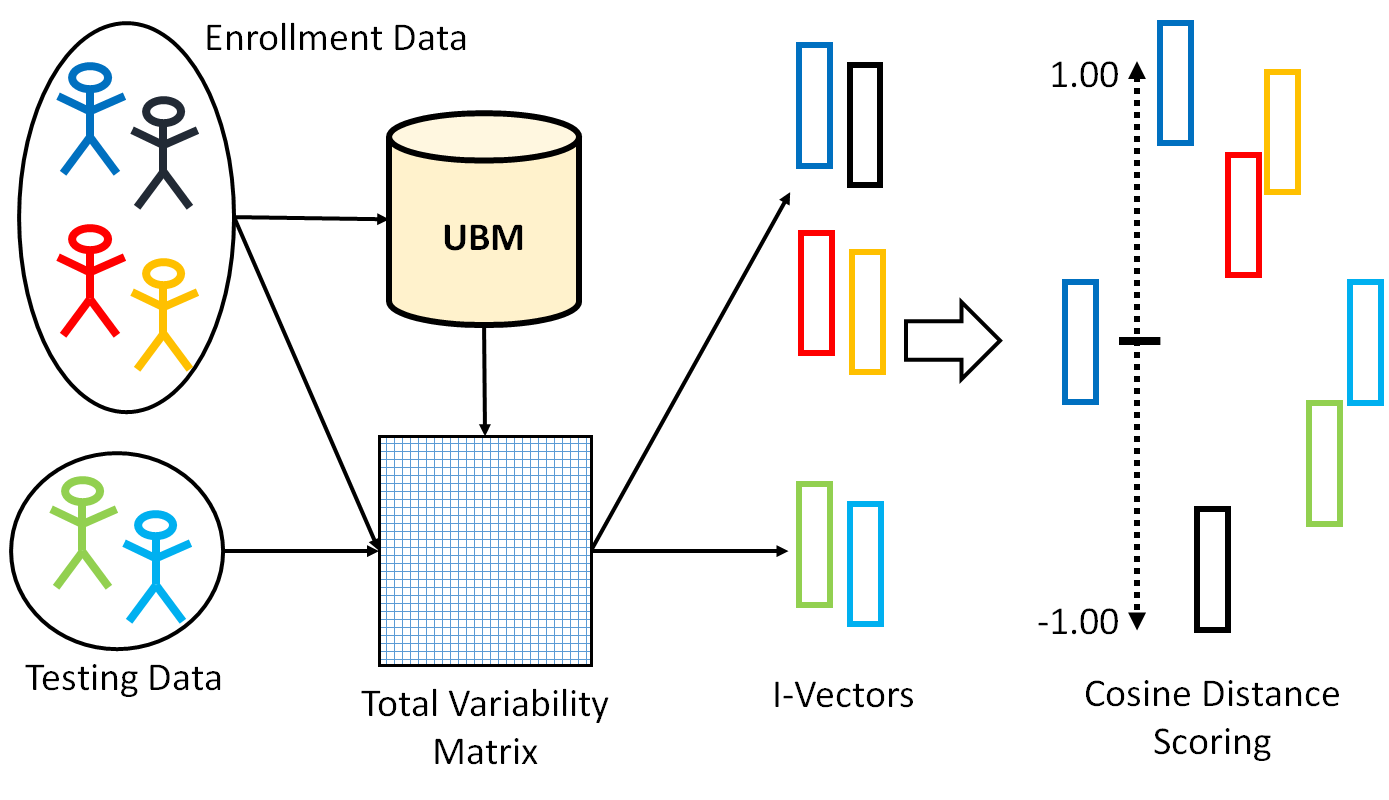
\includegraphics[width=0.9\linewidth,keepaspectratio]{figure2}
\caption[I-Vector Development]{Using the \acp{UBM} as an initialization, the enrollment and training data are transformed into \acp{IV}. This process is reliant on the creation of the total variability matrix randomly generated from the variances of the \acp{UBM} and refined by adaptation towards the means of the \acp{UBM}. The resultant \acp{IV} are pairwise evaluated to find the \ac{CD} between them to rank their similarity.}
\label{fig:iVector}
\end{figure}
%%%%%%%%%%%%%%%%%%%

A \ac{UBM} models the $f$-dimensional features by representing them with $C$ independent Gaussian mixtures \cite{Reynolds2000}. In general, increasing the number of mixtures captures more nuance, thereby potentially strengthening discrimination. The \acp{UBM} provide dimensionality reduction by taking a training dataset of $L$ epochs each with $f$ features each down to $C$ mixtures of $f$ features. As each feature has a mean $m$, variance $\sigma$, and weight $\rho$, reduction benefits are seen when $L > 3C$. The \acp{UBM} can be characterized according to:
\begin{equation}
\Omega_{c=1 \hdots C} =
\begin{cases}
m(c) \\
\sigma(c) \\
\rho(c)
\end{cases}
\end{equation}
Each parameter is a vector of length $f$ representing a given feature. Each \ac{IV} is the result of the \ac{EM} of the available \ac{UBM} and $M$.

The \acp{IV} are of length $l=Cf$ with many residual elements and are frequently further reduced by the speech community via \ac{LDA}. This process requires that the final \ac{IV} length be one less than the number of subjects $S$ or less given the constriants imposed by \ac{LDA}'s algorithm. Thus \acp{IV} final length, $l=min(S-1,Z)$, is frequently controlled by $S$ or $Z$, where $Z$ is on the order of 100s. The final \acp{IV} therefore represent a very dense and robust abstraction to an $l$ dimensional space. Within this space the similarity between two \acp{IV} can be found via any metric evaluation, often \ac{CD}.

%%%%%%%%%%%%%%%%%%%%%%%%
\subsection{Mathematics}
\label{2-mathematics}

The major components and steps to producing \acp{IV} are outlined in reverse starting with the resultant \acp{IV} and ending with the original \ac{JFA} technique. This includes sections on the \acp{TVM}, \acp{UBM}, \ac{MAP}, and \acp{GMM}.

\subsubsection{I-Vectors}

The critical component of equation \ref{eq-iVec_raw}, is the \ac{TVM} $T$. An evolution from the eigenvoice matrix used in \ac{JFA}, it captures all of the variances present in the \acp{UBM}. Generating $T$ from training data requires an iterative \ac{EM} approach reliant on feedback from the produced \ac{IV} $w$.
\begin{equation}
T = \begin{bmatrix} T_{1} \\ \vdots \\ T_{C}\end{bmatrix} =
\begin{bmatrix} A_{1}^{-1}*K_{1} \\ \vdots \\ A_{C}^{-1}*K_{C}\end{bmatrix}
\label{eq-finalT}
\end{equation}
The matrices of $A$ and $K$ represent the updated mean and variance of $T$. These updates are driven by $w$ and $T$ along with the static values of $N, \hat{F},$ and $\Sigma$. The superscript $H$ represents the Hermitian transpose.
\begin{align}
A_{c} =& \sum_{s=1}^{S}N_{s}(t)w^{-1}(t) \\
K_{c} =& \sum_{s=1}^{S}\hat{F}_{c}(s)*\big(w^{-1}(s)*T^{H}*\Sigma^{-1}*\hat{F}_{c}(s) \big)^{H}
\end{align}
The estimation of $w$ uses $T$ a $Cf \times Cf$ matrix. This matrix is formed from the \ac{BW} statistics $\hat{N}$ and $\hat{F}$, an $l \times l$ identity matrix $I$, and a model of the \ac{UBM} variances $\Sigma$. As the models are all independent $\Sigma$ is a diagonal $Cf \times Cf$ matrix of the true variances from the \acp{UBM} where as the \ac{BW} statistics are estimations of the mean $N$ and variance $F$.
\begin{equation}
w(s) = \left(I + T^{t}\Sigma^{-1}\hat{N}(s)T \right)^{-1} T^{t}\Sigma^{-1}\hat{F}(s)
\label{eq-fakeI}
\end{equation}
The \ac{BW} 0\textsuperscript{th} ($N$) and 1\textsuperscript{st} ($F$) order statistics are generated from the evaluation of the \acp{UBM} against the $L$ epochs in the training data. The higher order statistic must be offset by the preceding orders resulting in a centered 1\textsuperscript{st} order statistic $\hat{F}$. Each statistic models the $f$ features in each of the $C$ mixtures resulting in $C\times f$ matrices. Each epoch, $e$, from the full epoch set $t=1...L$ is evaluated to generate initial probabilities based on $\Omega$ for $N$ and $F$.
\begin{align}
\hat{N}(s)=& \begin{bmatrix} N_{1}(s) &  &  \\  & \ddots &  \\  &  & N_{C}(s) \end{bmatrix} \label{eq-newN} \\
\hat{F}(s)=& \begin{bmatrix} \widetilde{F}_{1}(s) \\ \vdots \\ \widetilde{F}_{C}(s) \end{bmatrix}  \label{eq-matStats}
\end{align}
\begin{align}
\widetilde{F}_{c}(s) =& F_{c}(s) - N_{c}(s)m_{c} \\ \label{eq:modF}
N_{c}(s) =& \sum_{t=1}^{L} P( c \mid e_{t} , \Omega ) \\
F_{c}(s) =& \sum_{t=1}^{L} P( c \mid e_{t} , \Omega ) e_{t} \label{eq-firstF}
\end{align}
This process resolves a suitable $T$ after approximately twenty iterations of equations \ref{eq-finalT} to \ref{eq-fakeI}. Notice that equations \ref{eq-newN} to \ref{eq-firstF} are needed only once to generate $T$. Creating \acp{IV} from the enrollment and testing data follows equation \ref{eq-iVec_raw} in a modified form. The resultant \ac{IV} $w$ will be a $l$ row vector where $l$ is a length defined during the creation of the initial estimate of $T$.
\begin{equation}
w = (M-m)T^{-1}
\end{equation}
The number of I-Vectors produced is based upon the enrollment targets $h$ and testing queries $q$, producing data on the order of $(h+q)\times l$. Therefore dimensionality reduction will not be significant if the data is partitioned such that $h+q \equiv L$.
\par
The \acp{IV} are finalized after applying \ac{LDA} to control for dependencies in the data. This process reduces their length from $l$ to $ l = min(S-1,l)$ elements based upon the transformation matrix produced by the \ac{LDA}. There are other approaches to normalize the \acp{IV} aside from \ac{LDA} which can be reviewed elsewhere \cite{Dehak2011}. These final \acp{IV} can be compared pairwise using \ac{CD} to determine similarity between enrollment targets and testing queries.
\begin{equation}
cos(\Theta_{w_{1},w_{2}})=\frac{w_{1}^{t}w_{2}}{\left\lVert w_{1} \right\rVert * \left\lVert w_{2} \right\rVert}
\end{equation}

%%%%%%%%%%%%%%%%%%%%%%%%%%%%%%%%%%%%%%%%
\subsubsection{Total Variability Matrix}

After the development of \ac{JFA} it was discovered that the iterative modeling process was not perfect at separating speaker, channel, and residual effects\cite{Dehak2011}. In fact the eigenchannel space was collecting information related to the subject when operating on specific utterances. \ac{JFA} was still considered state of the art, but its performance could be challenged by the total variability space. This space, formally the \ac{TVM}, was produced by using the first iteration of \ac{JFA} to generate a low-dimensional speaker- and channel-dependent matrix. As this matrix is the key component in generating \acp{IV} a detailed decomposition of its construct and applications is necessary. 

The initial form of the $T$ is $f \times C$, \acp{GMM} by features, shown in equation \ref{eq:ivBlock}. These parameters were dependent on each other and the training data. The speech community uses a definitive feature set \cite{Davis1980}, \acp{MFCC}, which evolved over time to become the gold standard \cite{Kinnunen2010}. This makes determining the number of features straightforward. Settling on an acceptable number of mixtures for the \ac{GMM} was more difficult given the trade-offs between classification and computational performance\cite{Glembek2011,McClanahan2015}.

In many studies the number of mixtures is on the order of a base 2 number, often being set to at least 2048 mixtures\cite{Garcia-Romero2011,Greenberg2014a}. The optimization for the number of mixtures was dependent on the best performance, but limited by the dimensions of the training data. Given a number of subjects $S$ each providing $u$ utterances the number of mixtures $C$ would need to be less than $S*u$ to prevent over-fitting.

\begin{equation}
\label{eq:ivBlock}
\begin{bmatrix} M_{1} \\ \vdots \\ M_{f} \end{bmatrix} =
\begin{bmatrix} m_{1} \\ \vdots \\ m_{f} \end{bmatrix} +
\begin{bmatrix} T_{1,1} & \dots & T_{1,C} \\ \vdots & \ddots & \vdots \\ T_{f,1} & \dots & T_{f,C} \end{bmatrix} *
\begin{bmatrix} w_{1} \\ \vdots \\ w_{C} \end{bmatrix}
\end{equation}

Critically, the \ac{TVM} was not implemented to mimic utterances, but to map them instead. The technique allowed \acp{IV} to be the weights controlling the inclusion of a column of features. In this manner it was possible that one column may contain the dominant features of a low pitched voice and a high pitched voice. If each of the $C$ columns of $T$ represent a unique component of the speakers, then the \ac{IV} $w$ would be binary. More likely is that the characteristics are spread across mixtures since emergent properties of speech are parameterized via the \acp{MFCC}.

Advancing this approach to \acp{EEG} may produce a reasonable algorithm for discrimination, but also allow for an understanding of why the discrimination occurs. This is entirely dependent on the chosen features, which are well established for speech, but still open for \acp{EEG}. Using a non-linear variation of \ac{MFCC} maintains the parameterization providing a closed set of features. With features bounded, experiments can then focus on finding an optimal size \ac{GMM} for the \ac{UBM} of \acp{EEG}.

Working down this chain, further incremental improvements can be made while gaining insight into the discrimination and grouping of \acp{EEG} in an unsupervised algorithm. While speech already knows the principal modes of their data, how to separate consonants, vowels, words, genders, and ages, such techniques do not meet the needs of the \ac{EEG} community.

%%%%%%%%%%%%%%%%%%%%%%%%%%%%%%%%%%%%%%%%%%%
\subsubsection{Universal Background Models}

As mentioned previously \acp{UBM} are sets of \acp{GMM} created from the features of continuous signals. The \acp{GMM} contextualize the varied speech signal segments as independent feature distributions regardless of the spoken text \cite{Reynolds2000}. This technique is suited to the problem of speaker recognition where the goal is to match subjects irrespective of data content. As this process is reliant on the likelihoods of features for a given model or subject sample, it can be used in an unsupervised manner to match and/or separate subjects.

The \ac{GMM} represents the core component of the \acp{UBM} which in turn makes them critical to the performance of \acp{IV}. Sets of Gaussian distributions ($M$) can be represented with a mean ($\mu$) and co-variance ($\Sigma$) drawn from each measurement or feature of the $D$-dimensional raw continuous data \cite{Reynolds2009}. This allows a likelihood calculation equation given a $D$-dimensional sample $x$ to compare against the model,
\begin{equation}
p(\bm{x}|\lambda) = \sum_{i=1}^{M}w_{i}g(\bm{x}|\bm{\mu}_{i},\bm{\Sigma}_{i})
\end{equation}
where $x$,$\mu$, and $\Sigma$ are vectors of length $D$ and $w_{i}$ corresponds to the weight of each mixture component where $\sum_{i=1}^{M}w_{i}=1$. The calculated likelihood provides an unsupervised estimation of the sample relating to the given model(s).

The $\lambda$ component of $p(\bm{x}|\lambda)$ represents the \ac{GMM} and associated parameters: $w_{i}$, $\bm{\mu}_{i}$, and $\bm{\Sigma}_{i}$. While the previous equation does not assign a subscript to $\lambda$ there would be $U$ \acp{GMM} which comprise the fully formed \ac{UBM}. Just as each \ac{GMM} attempts to determine the underlying states of the data, the \ac{UBM} requires depth to account for each class of signal.

As an example suppose one wants to know if the weather on a given day will require a heavy coat, a light coat, a raincoat, or no coat. If the temperature is below 45$^\circ$F a heavy coat is desired and if the temperature is above 70$^\circ$F no coat is necessary. In between these two temperatures a light coat may be necessary, but only if the day will be windy. At the same time, at any temperature above 45$^\circ$F with high humidity levels should warrant wearing a raincoat.

The \ac{GMM} representing raincoat would have a large variance for wind and temperature, but a small variance for humidity. The temperature means of heavy coat, light coat, and no coat would be unique. However, light coat and no coat would have a similar mean and variance for humidity and overlapping distributions for wind. Meanwhile, the heavy coat model would be insensitive to anything aside from temperature.
 
The weather conditions (humidity, temperature, and wind) become the three features modeled by the \acp{GMM}. Once four, or more, models are created they each categorize the required jacket. This full set becomes the UBM that provides a basis for evaluation of each day's weather. Given a weather report, the UBM would provide the likelihood of each jacket being the correct answer.

To calculate the likelihood for a multivariate normal distribution the follow equation is used, represented as the function $g(\bm{x}|\mathbf{\mu}_{i},\bm{\Sigma}_{i})$ from the prior equation,
\begin{equation}
g(\bm{x}|\bm{\mu}_{i},\bm{\Sigma}_{i}) = \frac{\text{exp}\Big\{-\frac{1}{2}(\bm{x}-\bm{\mu}_{i})'\bm{\Sigma}_{i}^{-1}(\bm{x}-\bm{\mu}_{i})\Big\}}{(2\pi)^{D/2}\lvert\bm{\Sigma}_{i}\rvert^{1/2}}
\end{equation}
From these equations estimations of underlying modes of the data can be found from which to build a suitable model. Two important assumptions are made in this process, the first is that each Gaussian mixture is independent of the other mixtures and the second is that the underlying modes can me adequately modeled with normal Gaussian distributions. These mixtures are therefore representing a unique hidden set of generators/states that create the resultant signal. Given that the number of hidden states is unknown, GMMs may produce mixtures with marginal weights or mixtures with redundant attributes.

%%%%%%%%%%%%%%%%%%%%%%%%%%%%%%%%%%%%%%%%%%%%%%%
\subsubsection{Maximum A Posteriori Parameters}

With a \ac{UBM} in place it is possible to tune the model toward specific subjects. The estimation of a subject specific model from a \ac{UBM} is called \ac{MAP} estimation\cite{Reynolds2009}. Just as with a \ac{UBM}, the statistics (weight, mean, and variance) of the subject are found from their data $S={\bm{s}_{t},...,\bm{s}_{T}}$. These expectations are derived from the prior model found from the \ac{UBM}, but operating on the subject specific data.
\begin{equation}
n_{i} = \sum_{t=1}^{T}\text{Pr}(i|\bm{s}_{t},\lambda_{\text{prior}})
\end{equation}
\begin{equation}
E_{i}(\bm{s}) = \frac{1}{n_{i}} \sum_{t=1}^{T}\text{Pr}(i|\bm{s}_{t},\lambda_{\text{prior}})\bm{s}_{t}
\end{equation}
\begin{equation}
E_{i}(\bm{s}^{2}) = \frac{1}{n_{i}} \sum_{t=1}^{T}\text{Pr}(i|\bm{s}_{t},\lambda_{\text{prior}})\bm{s}_{t}^{2}
\end{equation}
These are then able to adapt each $i$ mixture's weight, mean and variance. The amount of adaptation is based on the expectations and a chosen relevance factor $r^{\rho}$.
\begin{equation}
\hat{w}_{i} = \Big[\frac{\alpha_{i}^{w}n_{i}}{T}+(1-\alpha_{i}^{w})w_{i}\Big]\gamma
\end{equation}
\begin{equation}
\hat{\bm{\mu}}_{i} = \alpha_{i}^{m}E_{i}(\bm{s}+(1-\alpha_{i}^{m})\bm{\mu}_{i}
\end{equation}
\begin{equation}
\hat{\bm{\sigma}}_{i}^{2} = \alpha_{i}^{v}E_{i}(\bm{x}^{2})+(1-\alpha_{i}^{v})(\bm{\sigma}_{i}^{2}+\mu_{i}^{2})-\hat{\bm{\mu}}_{i}^{2}
\end{equation}
The adaptation coefficient is most often constant for all three statistics, but given unique labeling allowing for decoupling if necessary.
\begin{equation}
\alpha_{i}^{w,m,v} = \frac{n_{i}}{n_{i}+r^{\rho}}
\end{equation}
These new statistics not only provide subject specific models, but present a new set of models for discrimination. An example of this process is shown in \cref{fig:gmm_map}. The models themselves can be compared against each other to determine similarity in addition to evaluating them against new data samples.
\begin{figure}[ht]
\centering
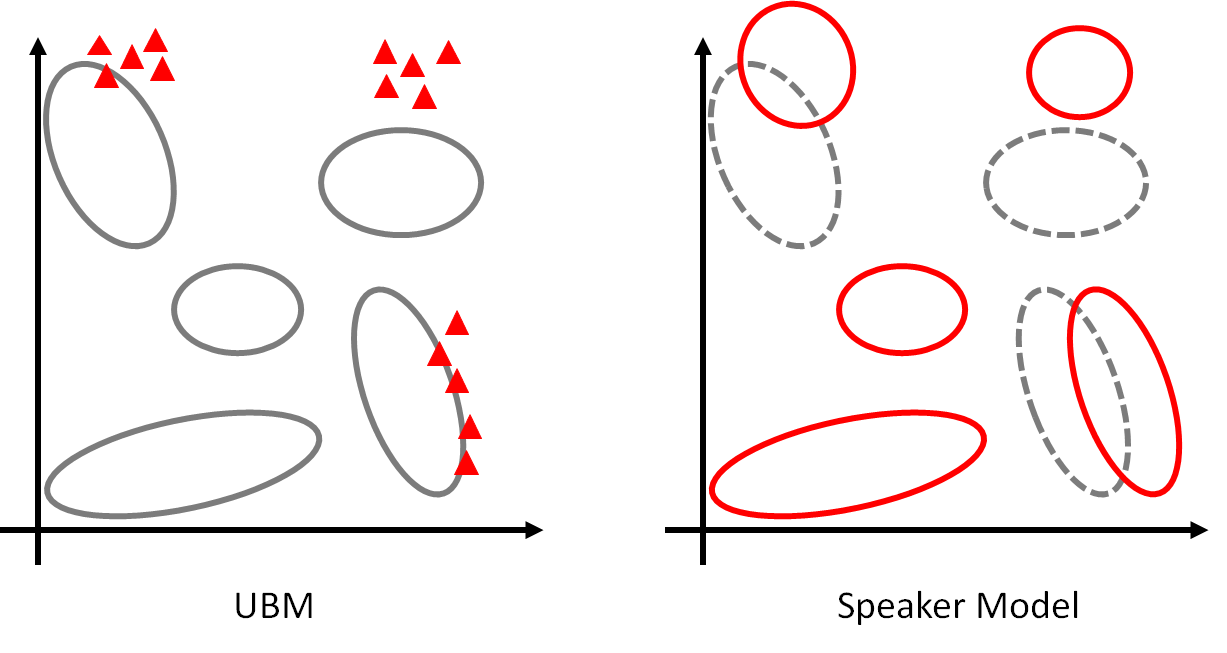
\includegraphics[width=0.9\linewidth]{gmm_map}
\caption[Example of MAP of GMM]{Results of MAP estimation when speaker data, red triangles, is applied to a UBM, gray mixtures.}
\label{fig:gmm_map}
\end{figure}

%%%%%%%%%%%%%%%%%%%%%%%%%%%%%%%%%%%%%%%
\subsubsection{Gaussian Mixture Models}
\label{sec:GMM}

Understanding how \acp{GMM} produce likelihoods for a given data sample $\bm{x}$ informs how each mixture's $\lambda$ is produced. The more accurate the parameters of $\lambda$ are for a given \ac{GMM}, the more insightful the resultant likelihoods. However, unless the parameters are known outright they must be deduced empirically. One of the more prevalent techniques for parameter estimation is \ac{MLE}\cite{Hyvarinen2001}.

The \ac{MLE} attempts to find a distribution that maximizes each of the $T$ training vectors $X=\{x_{1},...,x_{T}\}$
\begin{equation}
p(X|\lambda)=\prod_{t=1}^{T}p(\bm{x}_{t}|\lambda)
\end{equation}
this equation assumes that each component of the distribution is independent. This often turns out to be untrue, but is a necessary assumption to provide a functional solution. This function is non-linear as the product of all the training vector evaluations allows for one worsening likelihood to diminish any improvements gained from the remaining vectors. To avoid this problem, a variant of \ac{EM} can be used to estimate the parameters for each feature independently. This helps isolate the features, in the event that they are not independent, and provides the ability to directly improve the overall likelihood on a feature by feature basis.

With this each parameter of $\lambda$ can be estimated in an iterative manner with the following equations
\begin{equation}
\bar{w_{i}} = \frac{1}{T}\sum_{t=1}^{T}\text{Pr}(i|\bm{x}_{t},\lambda)
\end{equation}
\begin{equation}
\bar{\bm{\mu}_{i}} = \frac{\sum_{t=1}^{T}\text{Pr}(i|\bm{x}_{t},\lambda)\bm{x}_{t}}{\sum_{t=1}^{T}\text{Pr}(i|\bm{x}_{t},\lambda)}
\end{equation}
\begin{equation}
\bar{\bm{\sigma}}_{i}^{2} = \frac{\sum_{t=1}^{T}\text{Pr}(i|\bm{x}_{t},\lambda)\bm{x}_{t}^{2}}{\sum_{t=1}^{T}\text{Pr}(i|\bm{x}_{t},\lambda)}-\bar{\mu}_{i}^{2}
\end{equation}
these three equations provide updated values for the weights, means, and variances that can feed the next iteration of the EM algorithm. The \emph{a posteriori} probability Pr is found with the following equation
\begin{equation}
\text{Pr}(i|\bm{w}_t,\lambda)=\frac{w_{i}g(\bm{x}_{t}|\bm{\mu}_{i},\bm{\Sigma}_{i})}{\sum_{k=1}^{M}w_{k}g(\bm{x}_{t}|\bm{\mu}_{k},\bm{\Sigma}_{k})}
\end{equation}

%%%%%%%%%%%%%%%%%%%%%%%%%%%%%%%%%%%%%%%%%%%%%
\subsection{Success in Speech and Adaptation}

The deployment of \acp{IV} as a tool for speaker recognition/verification\cite{Kenny2015}, language detection\cite{Li2013a}, accent detection\cite{Behravan2015}, and speaker age\cite{Bahari2012} showed the growth and trust the speech community put into the algorithm. \acp{IV} were developed in 2011 at the \ac{CRIM} by Dehak, Kenny et al\cite{Dehak2011}. Prior to this work the group at \ac{CRIM} developed \ac{JFA} for use with speech data to address speaker and session variability\cite{Kenny2005}. Fundamentally, \acp{IV} were a natural extension of \ac{JFA}, but proved to be very effective as a feature preprocessing technique and their own classifier when paired with a simple metric like \ac{CD} \cite{Senoussaoui2010,Hasan2011}.

Fundamentally, evaluations of other \ac{ML} algorithms relied on tracking the sensitivity and specificity of each experiment and \acp{IV} were no different. In fact, they performed inline with other approaches achieving over 90\% sensitivity and 90\% specificity \cite{Greenberg2014a}. Given this development, the approach presented here represents the heart of the technique in as simple a manner as possible. The extensive use of \acp{IV} has produced a variety of augmentations, but it would have been unwise to start with a more complex system when transporting the technique to a new field of data. It was decided to minimize as many degrees of freedom as possible while developing \acp{IV} for \acp{EEG}.

Another problem in adapting this technique was that finding valid speech data was relatively easy. If someone was talking, producing sounds, they were likely producing valid data. However, that was not the case with \acp{EEG} which have a constant stream of data. It was not clear if \ac{EEG} recordings since background segments are not devoid of information, essentially all data is data of interest. This naturally leads to an increase in background signals in \acp{EEG} compared to speech. A sleep study may last for an entire night only to capture a brief 10 minute seizure. Easy for a clinician to correctly identify, but difficult for a \ac{ML} technique to recognize.

%%%%%%%%%%%%%%%%%%%%%%%%%%%%%%%%%%%%%
\section{Machine Learning Algorithms}

The breadth of potential algorithms, supervised and unsupervised, was too much to review in depth. Instead, a review of the most notable algorithms referenced in this section and those critical to the validation of \acp{IV} were reviewed in the following section. This was meant to provide necessary context to the present field of \ac{EEG} classification, but was not comprehensive to the rapidly developing realm of \ac{ML}. Similarly, a brief discussion of \ac{FA} was included given the frequent use of \ac{LDA} in supervised and unsupervised techniques and that \acp{IV} were predicated on \ac{JFA}.

%%%%%%%%%%%%%%%%%%%%%%%%%%%%
\subsection{Factor Analysis}
\label{sec:FA}

At a base level \acp{IV} reduced the dimensionality of data by finding the most influential features in the given training dataset. In a general sense this is similar to \ac{FA} which is used to perform \ac{BSS}, the decomposition of a signal into a linear representation of statistically independent components \cite{Hyvarinen2001}. While this was the goal, it is difficult to assure linear independence of all the components. As such the techniques are imperfect given the premise of being blind to the true nature of the data.

Two commonly used techniques to achieve \ac{BSS} are \ac{PCA} and \ac{ICA}. From these algorithms more advanced techniques, \ac{LDA} and \ac{QDA}, are capable of separating the components of different known classes. They are not able to operate blind, or unsupervised, as they require knowledge of the classes to define class dependent components. Knowing the dependent components they can then resolve the class independent components in an effort to discern the decisions surfaces between the classes. \ac{QDA} operates in a more generalized space allowing for separation of two or more classes compared to \ac{LDA} defining separability of a single class from the dataset. 

%%%%%%%%%%%%%%%%%%%%%%%%%%%%%%%%%%%%%%%%%%%%
\subsubsection{Principal Component Analysis}

\ac{PCA} finds the dominant components in a set of data by maximizing the variance of the given features \cite{Wold1987}. For a set of data $\bm{X}$ composed of $p$ columns of features and $n$ rows of observations there exists a vector $\bm{w}$ capable of maximizing the variance of a given feature.
\begin{gather}
\bm{V}=\frac{\bm{X}^{T}\bm{X}}{n} \\
\sigma^{2}_{w}=\bm{w}^{T}\bm{V}\bm{w}
\end{gather}
Here $\bm{V}$ represents the covariance matrix of the data matrix $\bm{X}$ which is used to find the eigenvectors that become $\bm{w}$. As eigenvectors are orthogonal to each other, they are each uncorrelated components and produce the $p$ principle components of the $\bm{X}$.

There are at most $n$ principle components representing unique weightings of the $p$ features. To find the true number of components, $q$, the number of zero or near zero eigenvalues, $e_{z}=p-q$, must be found. This linearly independent $q$-dimensional space represents the true decision surface of the observations. From these operations it becomes possible to define the critical features and unique observations from the data itself.

%%%%%%%%%%%%%%%%%%%%%%%%%%%%%%%%%%%%%%%%%%%%%%
\subsubsection{Independent Component Analysis}

\ac{ICA} separates individual signals from those collected by multiple receivers, commonly known as \ac{BSS} \cite{Hyvarinen2001}. The typical example is that of a cocktail party with an equivalent number of microphones and speakers. By using \ac{ICA}, it is possible to isolate each of the speakers using the data from all of the microphones. This example is referred to as the \textit{Cocktail Party Problem} and exists in many research areas including \ac{EEG} recordings.

A dataset contains the sequential samples, $t$, from each recording device and assumes there is a transformation matrix, $\bm{A}$, that turned the source signals, $\bm{s}$, into the captured output $\bm{X}$.
\begin{gather}
\bm{X} = \begin{bmatrix} x_{1}(t) \\ \vdots \\ x_{n}(t) \end{bmatrix}
\bm{A} = \begin{bmatrix} a_{1}{1} \dots a_{1}{n} \\ \vdots \ddots \vdots \\ a_{n}{1} \dots a_{n}{n} \end{bmatrix}
\bm{s} = \begin{bmatrix} s_{1}(t) \\ \vdots \\ s_{n}(t) \end{bmatrix}
\\
\bm{X} = \bm{A} \bm{S}
\end{gather}
From this output, the features of the recorded signals must be \emph{whitened} before the individual signals can be found. Whitening is a process that transforms the data into a matrix. $\bm{z}$ that is uncorrelated, but not assured to be independent. The approach is similar to \ac{PCA} in that it requires eigenvalue decomposition to produce the whitening matrix, $V$. The matrix $\bm{E}$ is found from the eigenvectors of $\bm{X}$ and the diagonal matrix $D$ contains the associated eigenvalue for each eigenvector.
\begin{gather}
\bm{z} = \bm{V}\bm{x} \\
\bm{V} = \bm{E}\bm{D}^{-\frac{1}{2}}\bm{E}^{T} \\
\bm{z} = \bm{V}\bm{A}\bm{s} = \hat{\bm{A}}\bm{s}
\end{gather}
Now the transformation matrix, $\hat{\bm{A}}$, contains only orthonormal components instead of the previous correlated components. This process is necessary as it constrains the solution sets when solving for the independent components.

The \emph{kurtosis} of a signal is one of the many ways to solve for the independent components after whitening. As the kurtosis supports the additive property, it provides a natural process for optimization the non-Gaussian portions of the signal. The expectations, E, of the random variable $y$'s second,variance, and fourth moment are used to find the `tailedness' of the distribution. With a normalized distribution the expectation of the variance would be 1, but for Gaussian distributions kurtosis would always be zero because the fourth moment is always $3(\text{E}\{y^{2}\})^{2}$. This is why the independent components must be non-Gaussian otherwise they cannot be separated out.
\begin{gather}
\text{kurtosis}(y) = \text{E}\{y^{4}\} - 3(\text{E}\{y^{2}\})^{2} \nonumber \\
\text{kurtosis}(s_{1}+s_{2}) = \text{kurtosis}(s_{1}) + \text{kurtosis}(s_{2}) \nonumber \\
\text{kurtosis}(\alpha s_{1}) = \alpha^{4}\text{kurtosis}(s_{1})
\end{gather}
When all the random variables are normalized the variance of $y$ is equal to $1$ which bounds the solution by the unit circle. This simplifies the solution to finding a vector that produces the largest amplitude of kurtosis for the given distribution. These kurtosis based dimensions indicate projections of non-Gaussian distributions which is where the suspected independent signals reside.
\begin{gather}
\lvert\text{kurtosis}(y)\rvert = \lvert q_{2}^{4}\text{kurtosis}(s_{1}) + q_{2}^{4}\text{kurtosis}(s_{2})\rvert
\end{gather}
There are other techniques for discerning the projection space of non-Gaussian distributions, Gram-Schmidt, \ac{ML} estimation, or negentropy, which focus separating independent non-Gaussian distributions. In all instances the mixing matrix $\bm{A}$ is chosen to be square to simplify the mathematics. The only constrains on the process, regardless of approach, are on the data being statistically independent and that the underlying signals are non-Gaussian distributions. These both require prior knowledge of the signals in the dataset otherwise the results of \ac{ICA} will be similar to those of \ac{PCA}, orthogonal uncorrelated feature vectors.

%%%%%%%%%%%%%%%%%%%%%%%%%%%%%%%%%%%%%%%%%%%%
\subsubsection{Linear Discriminate Analysis}

\ac{LDA} uses the mean and variance of each class in the data to build decision surfaces between the classes. This is achieved by maximizing the distance between the means $\bm{S}_{B}$ and minimizing the variances $\bm{S}_{W}$ of the features associated with the classes $K$. Original developed by Ronald Fisher, often called \textit{Fisher's Linear Discriminant}, it seeks to maximize the discriminant factor $J(\bm{w})$ by finding the vector $\bm{}w$ \cite{Izenman2008}.

Given two datasets containing $n_{i}$ observations of each class, a decision surface $\bm{w}$ can be found.
\begin{gather}
\bm{X}_{1} = \{\bm{x}_{1}^{1},...,\bm{x}^{1}_{n_{1}}\} \text{ , } \bm{X}_{2} = \{\bm{x}_{1}^{2},...,\bm{x}^{2}_{n_{2}}\} \nonumber \\
\bm{m}_{i} = \frac{1}{l_{i}}\sum^{n_{i}}_{j=1}\bm{x}^{i}_{j} \nonumber \\
\bm{S}_{B} = (\bm{m}_{1}-\bm{m}_{2})(\bm{m}_{1}-\bm{m}_{2})^{T} \nonumber \\
\bm{S}_{W} = \sum^{K}_{i=1} \sum^{n_{i}}_{j=1}(\bm{x}_{j}-\bm{m}_{i})(\bm{x}_{j}-\bm{m}_{i})^{T} \nonumber \\
J(\bm{w}) = \frac{\bm{w}^{T}\bm{S}_{B}\bm{w}}{\bm{w}^{T}\bm{S}_{W}\bm{w}}
\end{gather}
This can be expanded to handle multivarate data by expanding the definitions of $\bm{S}_{B}$ and $\bm{S}_{W}$. Here $\bar{\bm{m}}$ represents the mean of the observations $n_{i}$ across all classes in the training set. Then a sufficient $w$ can be found by maximizing $J(\bm{w})$ which occurs when $\bm{w}$ is an eigenvector of $\bm{S}_{W}^{-1}\bm{S}_{B}$.
\begin{gather}
\bm{S}_{B} = \sum^{K}_{i=1} n_{i}(\bm{m}_{i}-\bar{\bm{m}})(\bm{m}_{i}-\bar{\bm{m}})^{T} \nonumber \\
\bm{S}_{W} = \sum^{K}_{i=1} \sum^{n_{i}}_{j=1}(\bm{x}_{ij}-\bm{m}_{i})(\bm{x}_{ij}-\bm{m}_{i})^{T} \nonumber
\end{gather}
Classification based off \ac{LDA} requires an additional step to set thresholds for each class with respect to the resultant eigenvalues produced by $\bm{w}\cdot \bm{x}$. Through this metric many approaches can be used to distinguish between the $K$ classes in the multivariate data such as individual or one-versus-all classification.

The multivariate approach often assumes a common global covariance matrix $S_{X}$ to ensure that $S+{W}^{-1}S_{B}$ is diagonalizable. This assures that the eigevenvectors will be caused by the features within the data. To approximate a global covariance matrix the pooled within-class covariance matrix is scaled by the degrees of freedom between the observations and classes.
\begin{gather}
S_{X} = (n-K)^{-1}\bm{S}_{W}
\end{gather} 
This results in $K-1$ eigenvectors as diagonalizablity of a matrix does not ensure unique eigenvectors. In general, \ac{LDA} is frequently used to perform dimensonality reduction similar to \ac{PCA} based upon the eigenvalues associated with each eigenvector. Even without reviewing the eigenvalues, \ac{LDA} always produces one less feature dimension than classes to force discrimination upon the next eigenvector axis.

%%%%%%%%%%%%%%%%%%%%%%%
\subsection{Algorithms}

Numerous algorithms were introduced while reviewing the applications of \ac{EEG} recordings. The following section highlights the more common algorithms used in \ac{ML} and those to be compared against \acp{IV}. From training datasets the algorithms are able to classify unknown samples by providing a likelihood of a match or a discrete label if given labeled data. These introductions serve only to address the nature of the algorithm, unsupervised or supervised, the process of discrimination, and show the input parameters and type of classification produced.

%%%%%%%%%%%%%%%%%%%%%%%%%%%%%%%%%%%%
\subsubsection{Gaussian Classifiers}

Once created, \acp{GMM} can be used as the basis for discrimination. As discussed in section \ref{sec:GMM}, the data is broken down into a series of estimated Gaussian distributions. These distributions strive to model classes defined by the data. To identify new data, a likelihood score is generated based upon the distance between each model and the new data sample. Calculating the distance, and thus likelihood, can be done in a number of ways. Assuming the distributions are Gaussian in nature, the following equation provides the likelihood the point belongs with the model.

Here $x$ is the location in $d$ dimensional space with a known mixture modeled by its mean $\mu$ and co-variance $\Sigma$.
\begin{equation}
likelihood(x,\mu,\Sigma) = \frac{e^{-\frac{1}{2}(x-\mu)^{T}\Sigma^{-1}(x-\mu)}}{\sqrt{\lvert\Sigma\rvert(2\pi)^{d}}}
\end{equation}
This general form produces the likelihood a sample $x$ could come from a given mixture. The end result becomes a set of likelihoods of the known classes from which to draw a classification label. However, there is no assurance of a data sample exceeding 50\% likelihood of any of the classes.

This classifier functions based on the modeled distributions. If the \acp{GMM} are created via \ac{EM} or another clustering method the entire process is unsupervised. However, it is possible make the process supervised by knowing the class means and variances in advance or using labeled data to manual cluster the data. The evaluation of a likelihood based upon a distribution is a fundamental technique used by many \ac{ML} algorithms. It serves as a natural comparison point for \acp{IV} as a preliminary step in their development is to produce \acp{GMM}.

%%%%%%%%%%%%%%%%%%%%%%%%%%%%%%%%%%%%%%
\subsubsection{Naive Bayes Classifier}

\acp{NBC} make use of probabilities to classify based on discrete conditions. The classifier is built out from Bayes' Theorem which describes the probability of an event occurring given the current conditions. This approach requires knowledge about the events that inform the probabilities making it a supervised algorithm. The two class form of a \ac{NBC} is
\begin{equation}
\text{P}(A | B) = \frac{\text{P}(B|A)\text{P}(A)}{\text{P}(B)}
\end{equation}
which provides the likelihood of $A$ given $B$. In this equation $\text{P}(A)$ and $\text{P}(B)$ represent the independent probabilities of events $A$ and $B$ and the probability of $B$ given $A$ is given as $\text{P}(B|A)$. This expands to multiple conditions $T$ by taking into account the likelihoods of each possible condition with
\begin{equation}
\text{P}(A_{i} | B ) = \frac{\text{P}(B|A_{i})\text{P}(A_{i})}{\sum_{i}^{T}\text{P}(B|A_{i})\text{P}(A_{i})}
\end{equation}
The expansion of the unitary case shows that as the number of conditions increases probabilities for each condition with respect to each class are needed. In a sense the conditions could be features representative of classes or the classes themselves.

The approach is a natural tool for evaluating any modeling technique that produces discrete probabilities assuming they are all independent. Since this cannot always be assumed the technique's performance is dependent on adequate feature selection and class separation. The outcome is a probability of the test event or class occurring that is bounded on $(0\%-100\%)$.

%%%%%%%%%%%%%%%%%%%%%%%%%%%%%%%%%%%%%%%%%%%%%
\subsubsection{K-Nearest Neighbor Classifier}

A \ac{KNN} classifier uses labeled datasets to assume the class of an unknown sample. This approach is similar to using \acp{GMM}, but \ac{KNN} can only operate with labeled data. Given the $k$ closets neighbors class, the unknown sample is labeled as the highest counted class. The algorithm relies on mapping distances between the data points in their $f$ dimensional feature space \cite{Cover1967}.

Determining the distance between unique samples provides flexibility in handling non-Gaussian distributions. Unlike \acp{GMM} classifiers and similar to \acp{NBC}, this algorithm operates directly on the data and not through a model when fed training data. The trade-off becomes having enough data and selecting a sufficient value of $k$ to produce acceptable classifications. The previous two algorithms relied on the statistics drawn from the training data, but \ac{KNN} is directly dependent on samples in the training data.

The simplistic nature of and ease of conceptulizing lead \ac{KNN} to be used in a variety of experiments as a comparative benchmark \cite{Wulsin2011,Acharya2012}.

%%%%%%%%%%%%%%%%%%%%%%%%%%%%%%%%%%%%%%%
\subsubsection{Support Vector Machines}

Another kernel based classifier, \acp{SVM}, creates a hyperplane between a target class and all other data. The use of a kernel allows linear and non-linear decision surfaces to be transformed onto a hyperplane for discrimination. This hyperplane maximizes the distance between a target cluster and a non-target cluster \cite{Cortes1995}. Development of the technique stemmed from considering two normal distributions $\bm{N}_{1}:m_{1}, \Sigma_{1}$ \&  $\bm{N}_{2}:m_{2}, \Sigma_{2}$ and an target location $x$.
\begin{equation}
F_{sq}(x)=\text{sign}\Big[ \frac{1}{2}(x-m_{1})^{T}\Sigma_{1}^{-1}(x-m_{1})-\frac{1}{2}(x-m_{2})^{T}\Sigma_{2}^{-1}(x-m_{2})+\text{ln}\frac{\lvert\Sigma{2}\rvert}{\lvert\Sigma_{1}\rvert}\Big]
\end{equation}
In this case $F_{sq}(x)$ resolves to a positive sign indicative point $x$ is in $\bm{N}_{1}$ and a negative sign for $\bm{N}_{2}$. From this initial equation may variations developed to address non-normal distributions and how to simplify the equation by approximating $\Sigma_{1}\approx\Sigma_{2}$.

Results of \acp{SVM} are a binary one-versus-all classification. This provides no way to produce clusters of data nor known the strength of the classifications. As with the other classifiers it builds the hyperplane used for separation from a labeled training set, making it a supervised classifier. As it seeks to maximize the space between clusters additional data is most beneficial when it represents boundary conditions of each class. It has been used on \acp{IV} in the speech community \cite{Cumani2017} and numerous \ac{EEG} classification tasks \cite{Wulsin2011,Radha2014,Brigham2010}.

%%%%%%%%%%%%%%%%%%%%%%%%%%%%%%%%%
\subsubsection{Dirichlet Process}

A \ac{DP} allows for distributions of distributions to be built in an unsupervised manner. The process produces random variables $G_{K}$ as sub-distributions from the full dataset's distribution $G_{0}$ given a concentration parameter $\alpha$. In this manner an unlimited number of distributions can be produced from a closed dataset containing $T_{1}...T_{K}$ partitions\footnote{A partition of $\Theta$ defines a collection of subsets whose union is $\Theta$. A partition is measurable if it is closed under complementation and countable union.} of the data $\Theta$\cite{Gershman2012}.
\begin{gather}
G \approx \text{DP}(\alpha,G_{0}) \\
\Big[ G(T_{1}),...,G(T_{K}) \Big] \approx \text{Dir}(\alpha G_{0}(T_{1}),...,\alpha G_{0}(T_{K}))
\end{gather}
Generating new distributions in this manner assures that the average distribution properties are maintained. Those distributions with large $\alpha$ will contribute more heavily, but have a greater likelihood of exemplifying the full dataset's true distribution. Through iterative measures it is possible to produce distributions that separate into naturally defined classes based on the dataset alone.

The clustering of the data occurs via the atoms at each level. An atom is a model of the statistical patterns of some phenomena in the data. At the lowest clustering level only atoms relevant to that level are present, but the next highest level contains these atoms plus their own atoms. Building up towards the highest clustering level means collecting all the atoms along the way. By sharing the atoms across the dataset, it becomes possible to then map similarities based upon the mixture of these atoms at each level \cite{Teh2006}.

The version used in Wulsin et al.\cite{Wulsin2012}, \ac{HDP}, allows distributions to be drawn across multiple levels of the data at once. This exemplifies the use case of a \ac{DP} for clustering data on multiple levels with minimal prior knowledge. Wulsin built clusters at each level of the data (subject, seizure, and channel) so the knowledge was about the structure of the data and not the contents of the data. This is similar to \acp{IV} as features are clustered in the \acp{GMM} and then the resultant samples are clustered based on the feature models.

%%%%%%%%%%%%%%%%%%%%%%%%%%%%%%%%%%%%%%%%%%
\subsubsection{Artificial Neural Networks}

By applying the functional structure of brain neurons, an algorithm that behaves as a \ac{NN} can be trained to perform non-linear classification. Each node in the network takes in information from the preceding layer, evaluates an equation to determine its state, and then contributes this activation to the ensuring layer. The connections between nodes have their own weights and the number and depth of layers is based upon the needs of the network. The algorithms referenced thus far included \acp{DBN}, \acp{RBFNN}, \acp{MLPNN}, and \acp{MLPNN} represent a small sample of breadth of \acp{NN}.

Depending on the type of data and intended classification goal one \ac{NN} may perform better than another. The trade-offs between the algorithms stem from the characteristics of the data related to the number of classes and any temporal relationships. At the crux of these algorithms is the need for a large diverse amount of labeled data. Like other algorithms, they learn directly through each sample of data which enables them to be non-linear classifiers. The training methodology is driven by reducing the error in the training dataset through adjusting the weights connecting the nodes and the biases of activation in each node. The complexity of the problem to be solved is often matched by the complexity of the \ac{NN}.

Of interest to the development of \acp{IV} is a \ac{LSTMNN} adaptation capable of quantifying the similarity between two inputs \cite{Mueller2016}. By training on ranked input vectors, in the case of Mueller et al. \cite{Mueller2016} sentences, the algorithm can learn to produce a discrete similarity score. This approach is highly dependent on the initialization parameters and the quality and quantity of training data available given the need to operate on variable length input vectors that represent the same classification.

%%%%%%%%%%%%%%%%%%%%%%%%%%%%%%%%%%%%%%%%%%
\subsubsection{X-Vectors}

The \ac{IV} methodology was improved upon while this work was ongoing by research in the speech community that augmented it with a \ac{DNN} \cite{Snyder2017}. This combined system used \acp{IV} and embeddings from a feed-forward deep neural network (the x-vectors) to surpass both of their individual speaker verification performances. The premise of the x-vectors was to utilize the post-statistics pooling layers of the \ac{DNN} to generate feature vectors. The first embedding was taken from the first affine layer after the statistics pooling and second embedding was taken from the affine layer that received the output of a ReLU (rectified linear units) layer driven by the previous embedding. This made the first embedding a linear representation of the speaker's statistics and the second embedding a non-linear representation of the same statistics. The embeddings and \acp{IV} are evaluated using the same process of \ac{LDA} followed by length normalization and \ac{PLDA} to produce the classification scores.

The original research group further refined the technique to the point that it surpassed its \ac{IV} counterparts \cite{Snyder2018}. These results were promising for advancing speaker recognition on text-independent datasets, where \acp{IV} had been the standard classification technique. However, the x-vector approach is a supervised \ac{ML} algorithm which relied on speaker labels to build the embeddings from the training dataset before generating the embeddings from the test dataset. They are clearly superior to \acp{IV} for speaker/subject recognition, but this approach would be reliant on clinical annotations to expand subject recognition. Additionally, the computational requirements of x-vectors is orders of magnitude beyond that of the presented \ac{IV} technique, as the original work by Snyder et al \cite{Snyder2017} utilized 4.4 million parameters over all layers of the \ac{DNN}.